\chapter{Results and discussion}

\section{Data exploration}
As described in Chapter 3, the data for the experiments is taken from Twitter. It was extracted and pre-processed by \cite{preotiuc-pietro_automatically_2019} and further enhanced with the labels for complaint severity by \cite{jinModelingSeverityComplaints2021}. What follows are the key findings from the exploratory data analysis performed. Some minor differences in the distribution of the Tweets across the domains are observed between the latest version of the dataset available in the public domain\footnote{\url{https://archive.org/details/complaint_severity_data}} and the distribution described in the original paper. Since the variations are minor (0.5 to 2\%), any potential impact on the model performance should be insignificant in the context of the objectives of the experiments. Refer \ref{sec: apdxa_fulldataset} for the full breakdown of the dataset used here.

\subsection{Domain and class distribution}
\begin{figure}[htb]
    \centering
    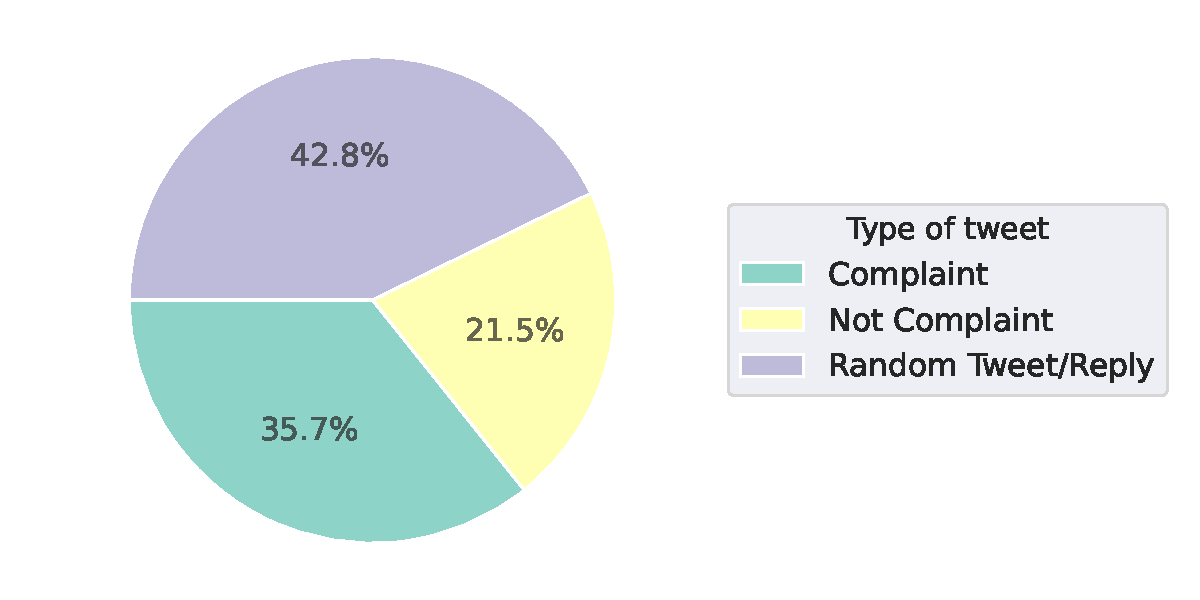
\includegraphics[width=9cm]{figures/compl_non_random_dist.pdf}
    \vspace*{-3mm}
    \caption{Illustrates the distribution of Tweets categorised as 'complaints' and 'not complaints', with random 'Tweets / replies' shown separately.}
    \label{fig: compl_non_random_dist}
\end{figure}


All Tweets categorised as complaints are assigned \texttt{label:1}, while Tweets that do not constitute complaints are assigned \texttt{label:0}. In terms of class distribution, the dataset is skewed towards 'not complaint' Tweets, as depicted in Figure \ref{fig: compl_non_random_dist}, where \texttt{label:1} represents 35.7\% and \texttt{label:0} represents 64.3\% of the dataset. Random Tweets and replies with \texttt{label:0} were added by the authors of \cite{preotiuc-pietro_automatically_2019} to ensure a more representative dataset. This approach aligns with the real-world scenario where complaint-related posts form a smaller proportion within an organization's social media Tweets and posts. Additionally, this strategy has the potential to enhance the model's ability to generalize effectively during the finetuning process.\\

\begin{figure}[htbp]
    \centering
    \captionsetup{font=small}
    \begin{subfigure}{0.49\textwidth}
        \centering
        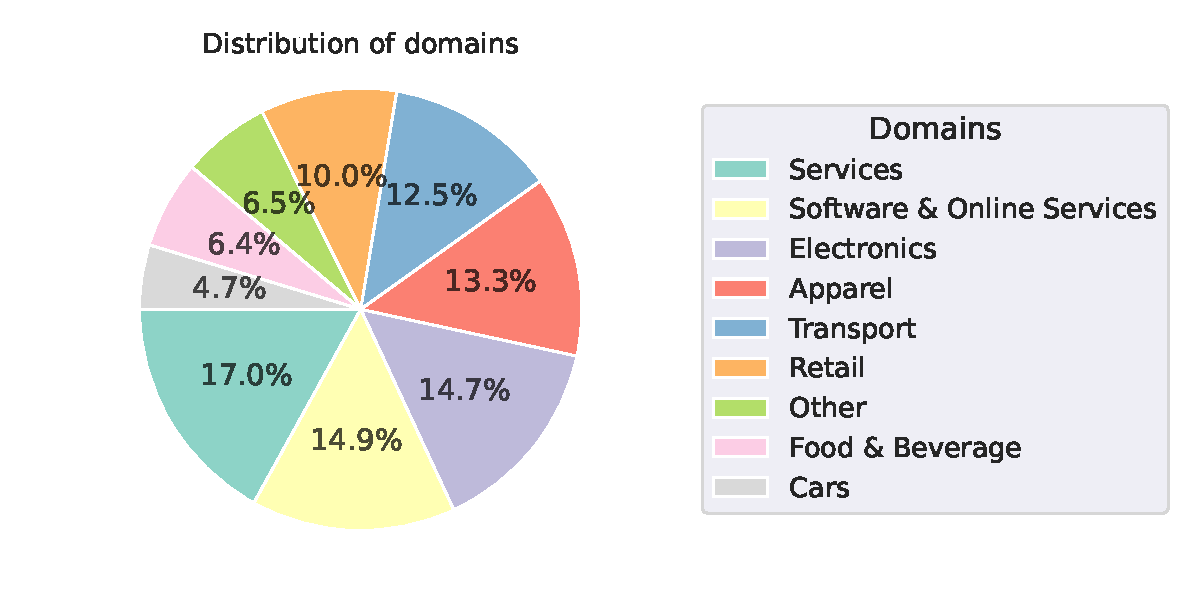
\includegraphics[width=\linewidth]{figures/domain_dist.pdf}
        \caption{Proportion of each domain}
        \label{fig: domain_dist_pct}
    \end{subfigure}
    \hfill
    \begin{subfigure}{0.49\textwidth}
        \centering
        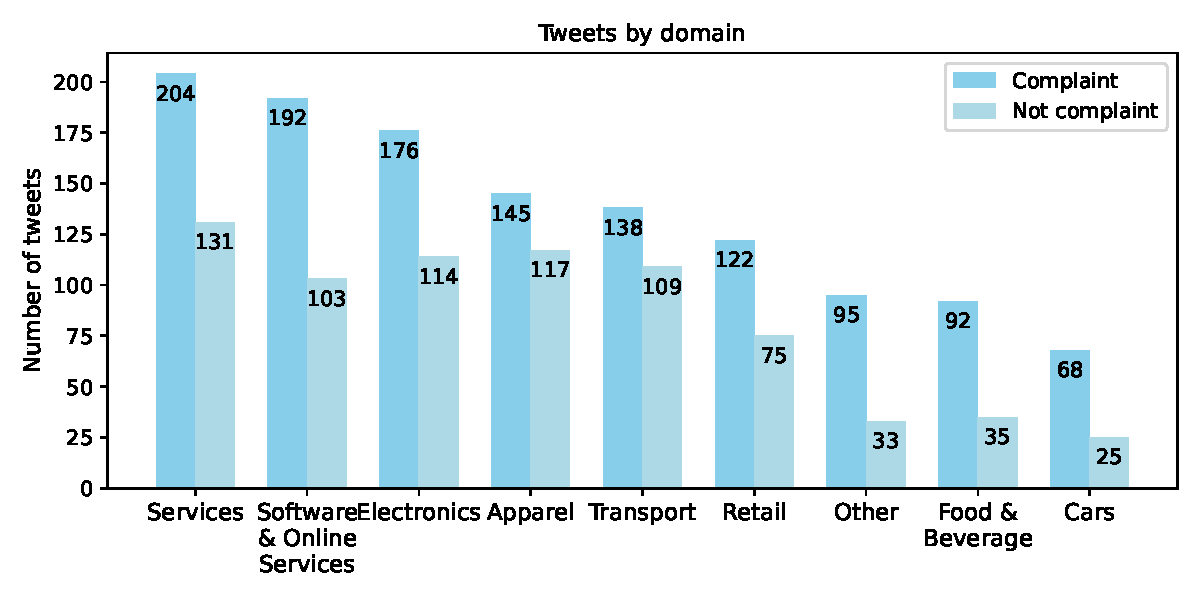
\includegraphics[width=\linewidth]{figures/domain_counts_bar_norandom.pdf}
        \caption{No. of Tweets for each domain}
        \label{fig: domain_dist_count}
    \end{subfigure}
    \caption{Shows the distribution of the domains used in the dataset}
    \label{fig: compl_main_dist}
\end{figure}

The dataset comprises domains encompassing both complaint-related Tweets and non-complaint Tweets. Figure \ref{fig: domain_dist_pct} illustrates the distribution of domains, with the top 3 categories being services, software, and electronics, collectively constituting nearly 50\% of the Tweets. A key observation from Figure \ref{fig: domain_dist_count} is the prevalent class imbalance within most domains, accompanied by relatively low tweet volumes within each domain. The implications of these observations on predictions are analyzed in Experiments set 2 and elaborated upon later in this chapter.

\begin{figure}[htbp]
    \centering
    \captionsetup{font=small}
    \begin{subfigure}{0.49\textwidth}
        \centering
        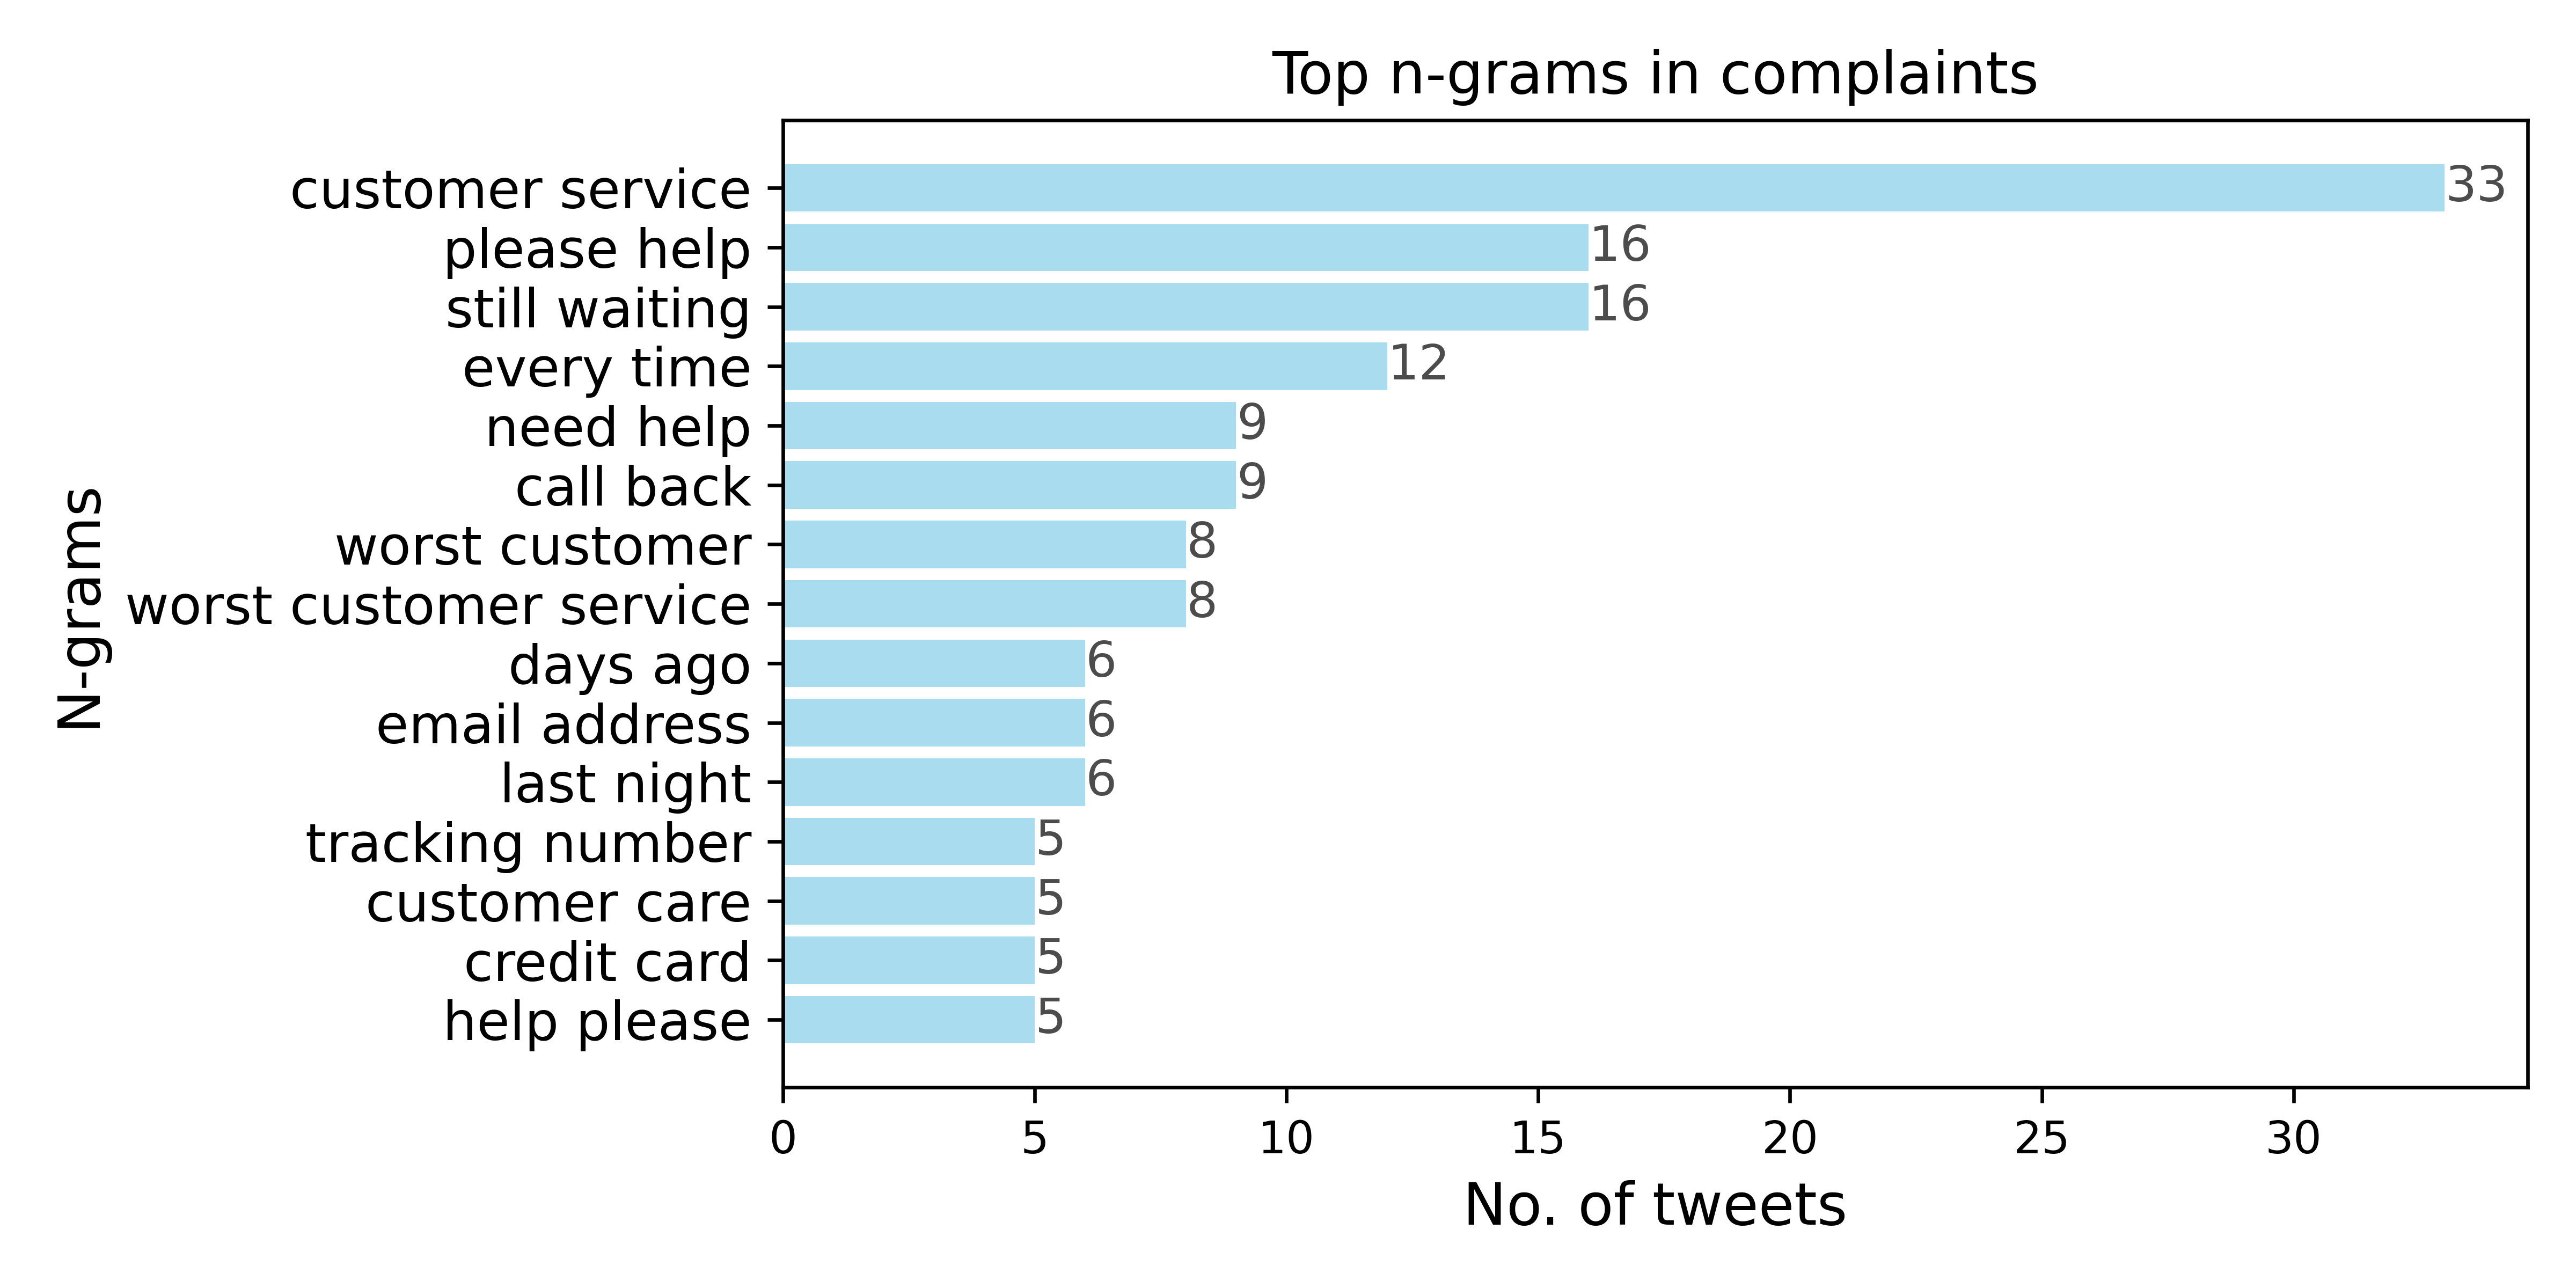
\includegraphics[width=\linewidth]{figures/top_ngram_horiz_bar.png}
        \caption{Top n-grams}
        \label{fig: top_ngrams}
    \end{subfigure}
    \hfill
    \begin{subfigure}{0.49\textwidth}
        \centering
        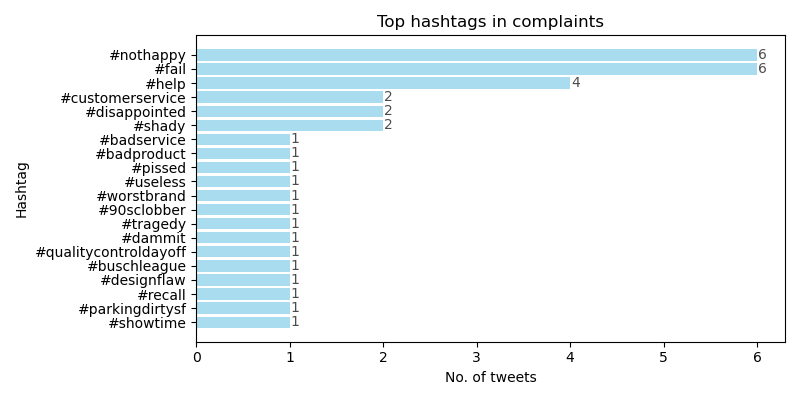
\includegraphics[width=\linewidth]{figures/top_hash_horiz_bar.png}
        \caption{Top hashtags}
        \label{fig: top_hashtags}
    \end{subfigure}
    \caption{Top phrases as n-grams(excl. unigrams) and hashtags in the complaint Tweets.}
    \label{fig: top_ngrams_hashtags}
\end{figure}

\subsection{Linguistic analysis}
Delving deeper into the language used in Twitter complaints, the top phrases are analysed by extracting n-grams. As depicted in Figure \ref{fig: top_ngrams}, common phrases in the complaint Tweets either convey an exepectation for resolution (such as "please help" and "need help") or express frustration (like "still waiting," "worst customer service," and "call back"). Others cover  broader customer service themes (for instance, "tracking number" and "customer care"). To elaborate further, sample Tweets with these phrases are shown below. They showcase various characteristics previously discussed, including instances of Face Threatening Acts, feelings of betrayal, altruistic behaviour (warning others), as well as elements like sarcasm. These findings align with the definition of a complaint and the intentions of the speaker as outlined in previous chapters.\\

\textbf{Examples for expectation of rectification}
\begin{quote}
    \textit{"hey chrysler cares i'm the one with the 2011 200 \textbf{need help} with the heating . inside the car it's really strange"}
\end{quote}
\begin{quote}
    \textit{"can someone \textbf{please help} me ? i've already sent a dm ."}
\end{quote}
\textbf{Examples for expression of frustration}
\begin{quote}
    \textit{"\textbf{worst customer service} experience with <user> <user> <user> . never been treated with such contempt"}
\end{quote}
\begin{quote}
    \textit{"on hold with <user> an hour just to get told to \textbf{call back} another day . hell yeah"}
\end{quote}
\begin{quote}
    \textit{"\textbf{worst customer service} to-date <user> in greensboro off wendover . avoid this place and let's show them we have other choices . \#otherchoices"}
\end{quote}

Examination of the hashtags within the complaint Tweets as shown in Figure \ref{fig: top_hashtags} points to their usage predominantly as a means of conveying frustration. Hashtags such as \texttt{\#nothappy}, \texttt{\#fail}, and \texttt{\#disappointed} are examples. Consequently, in addition to expressing dissatisfaction, these hashtags also communicate negative sentiments. Apart from these particular types of hashtags, various brand-specific or product-specific hashtags are used. As per Twitter\footnote{\url{https://help.twitter.com/en/using-twitter/how-to-use-hashtags#}}, users utilize the symbol "\#" (hashtag) preceding a keyword or phrase significant to the context in their tweet to classify those Tweets, facilitating their visibility in Twitter searches. Clicking or tapping on a hashtagged term within any message reveals additional Tweets containing the same hashtag. Hashtags can be inserted at any point within a Tweet. Frequently, words marked with hashtags that attain significant popularity transform into trending topics. \\

However, the volume of Tweets which include hashtags, particularly in the context of complaints is relatively low. Out of a total of 459 Tweets, only 149 complaint Tweets incorporate hashtags, constituting roughly 12\% of all complaint-related Tweets. When excluding random Tweets and replies, the Tweets that are not complaints containing hashtags amount to only 67 instances. There is an average of 1.56 hashtags in Tweets containing at least one. While the inclusion of hashtags may offer some assistance to the predictions by the models, their overall impact on the fine-tuning process could be quite limited due to their low prevalence in the dataset.\\

\subsection{Sentiment analysis}
\begin{figure}[htb]
    \centering
    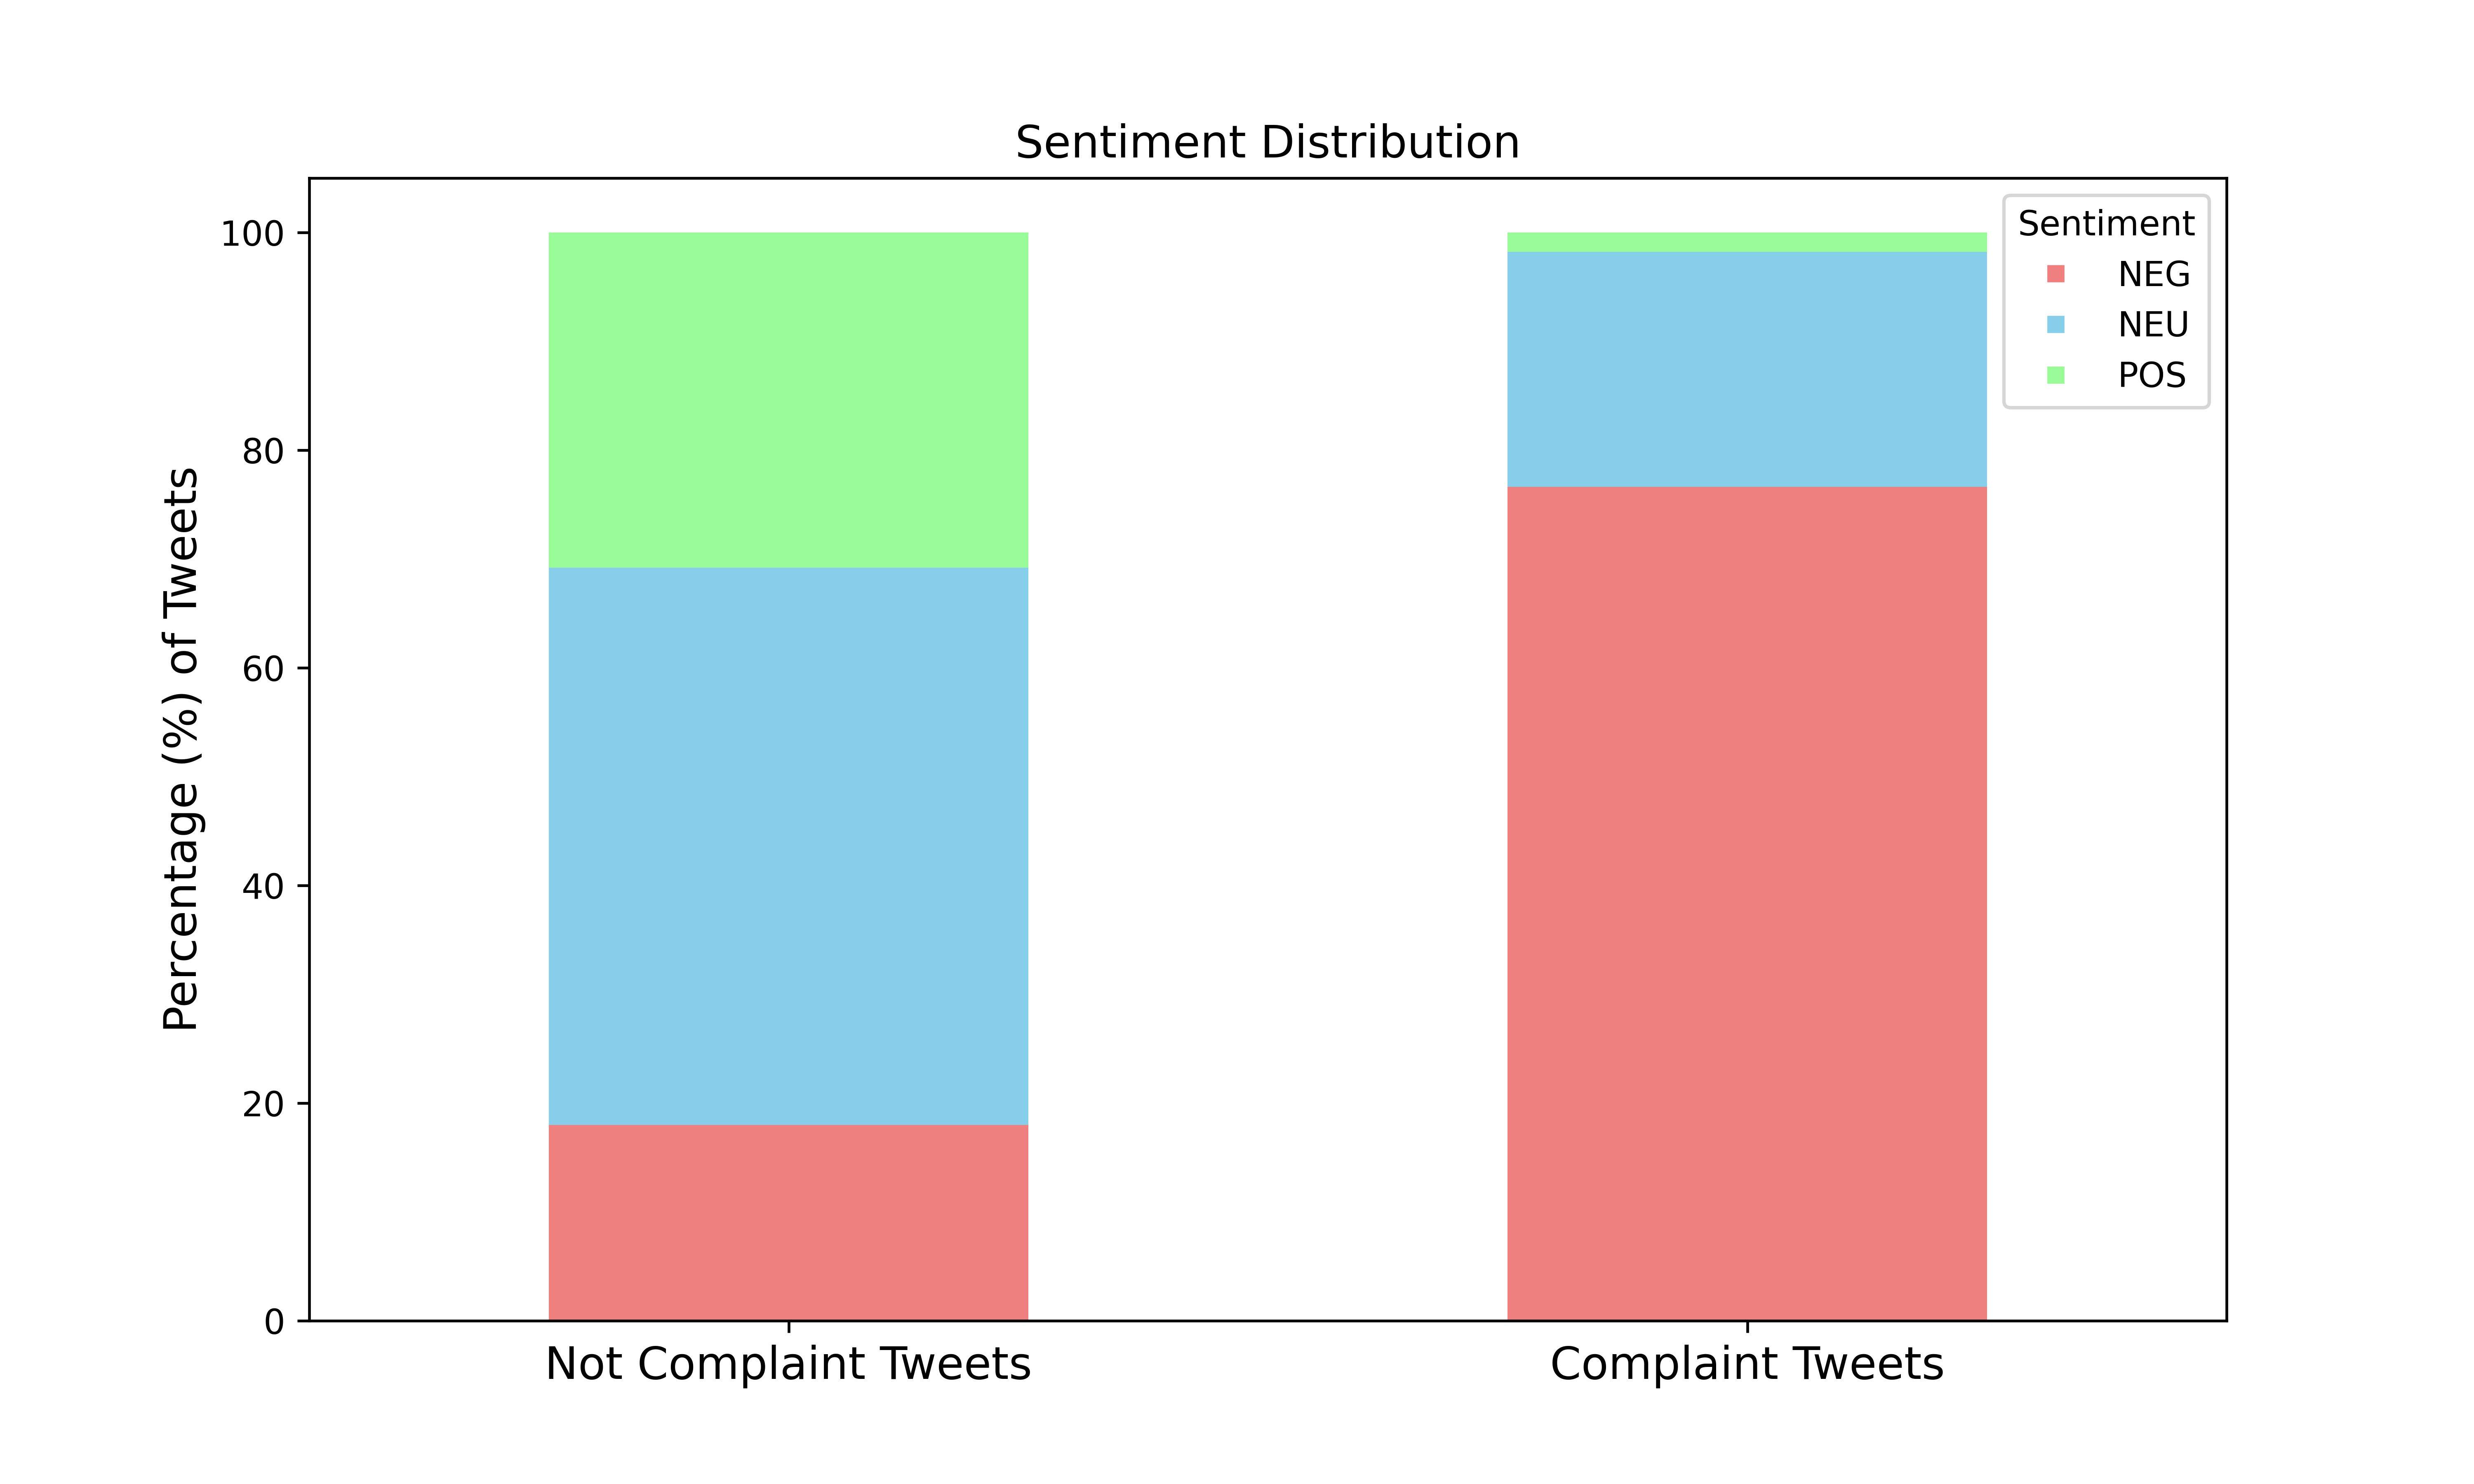
\includegraphics[width=12cm]{figures/sentiment.png}
    \vspace*{-3mm}
    \caption{Distribution of positive, negative and neutral sentiments in the Tweets.}
    \label{fig: sentiment}
\end{figure}

The act of complaining typically involves conveying a sense of negativity. Sentiment analysis was conducted on the dataset using  pysentimiento's library \cite{perezPysentimientoPythonToolkit2021} and the results are in Figure \ref{fig: sentiment}. As expected, the majority of complaint-related Tweets convey some form of negative sentiment, while approximately a quarter of them exhibit a neutral sentiment. A few examples of such neutral sentiment Tweets are as follows: \textit{"anyone know what's up with the geforce 500 series 580 gpx driver 275.33"} and \textit{"hi m order is 913181 did you revise the money ? if you did .. how about the shipping ?"}. These instances appear to involve raising a complaint while simultaneously posing a question that doesn't overtly express negative sentiment. While an undercurrent of dissatisfaction is evident, the situation has not escalated to the point requiring language which explicitly expresses negative sentiment.\\

Next, the small number of positive Tweets among the complaints were analysed. It was found they mostly involved sarcasm or where the consumer was expressing their liking for a product with the hope this could quicken the resolution process. Some of the example Tweets for these scenarios are: \textit{"hello i have a 2012 impreza and i love it . my driver seat back is broken down after 1 year and 12000 miles 32000 total 2nd owner"} and \textit{"i love waiting at mcdonalds for 15 minutes just for some semi-good ice cream <url>"}. For Tweets that were not complaints, the majority of them expressed neutral or positive sentiments.

\subsection{Key statistics}
% key statistcis table
\begin{table}[htbp]
    \captionsetup{font=small}
    \small
    \centering
    \begin{tabularx}{\textwidth}{|l|X|X|X|X|}
        \hline
        \rowcolor[gray]{0.7}
        \textbf{Statistic}              & \textbf{All Tweets} & \textbf{Complaints} & \textbf{Not Complaints} & \textbf{Random} \\
        \hline
        Number of Tweets                & 3449                & 1232                & 742                     & 1475            \\
        \rowcolor[gray]{0.9}
        Number of unique Tweets         & 3395                & 1232                & 737                     & 1427            \\
        \hline
        \hline
        Max tweet length (char.)        & 297                 & 297                 & 266                     & 144             \\
        \rowcolor[gray]{0.9}
        Min tweet length (char.)        & 1                   & 7                   & 6                       & 1               \\
        Mean tweet length (char.)       & 77.8                & 96.7                & 70.2                    & 65.8            \\
        \rowcolor[gray]{0.9}
        Median tweet length (char.)     & 79.0                & 98.0                & 68.0                    & 63.0            \\
        Standard Deviation tweet length & 41.4                & 40.5                & 38.9                    & 37.5            \\
        \hline
        \hline
        Total number of tokens          & 55169               & 24260               & 10839                   & 20070           \\
        \rowcolor[gray]{0.9}
        No. of unique tokens            & 7937                & 4031                & 2558                    & 4386            \\
        Maximum tokens                  & 57                  & 57                  & 55                      & 39              \\
        \rowcolor[gray]{0.9}
        Minimum tokens                  & 1                   & 2                   & 1                       & 1               \\
        Mean tokens                     & 16.0                & 19.7                & 14.6                    & 13.6            \\
        \rowcolor[gray]{0.9}
        Median tokens                   & 16.0                & 20.0                & 14.0                    & 13.0            \\
        Standard Deviation for tokens   & 8.6                 & 8.4                 & 8.0                     & 8.0             \\
        \hline
        \hline
        Mean punctuation count          & 3.4                 & 3.9                 & 2.7                     & 3.3             \\
        \hline
    \end{tabularx}
    \caption{Statistics of Tweets in the dataset.}
    \label{tab: tweets_statistics}
\end{table}

Finally, examining some of the key statistical measures from the Tweets dataset in Table \ref{tab: tweets_statistics}, we observe that complaint Tweets tend to exhibit a higher average tweet length, both in terms of characters (96.7) and tokens (19.7). In contrast, random Tweets and replies have a token count lower by 30\%, while non-complaint Tweets possess an average of 25\% fewer tokens than complaint Tweets. This disparity may stem from individuals employing diverse linguistic expressions to express their dissatisfaction or disappointment, or to communicate a Face Threatening Act directed at the subject of the complaint.

\section{Experiment set 1 results: Comparision of model performance}
As described in the previous chapter, to compare the performance of the models a nested cross-validation approach was adopted. The cross-validation method finetuned the models using 4 learning rates, $l\:\epsilon\:[1e-5, 5e-6, 5e-5, 3e-5]$ with the best-performing model based on the F1 score being selected for the testing for each iteration of the outer loop. \\

\subsection{Best predictive performance}
The best-performing model was found to be BERTweet with a mean F1 score of 0.908 (sd: $\pm$0.01), accuracy of 0.934 (sd: $\pm$0.01) and ROC AUC of 0.931 (sd: $\pm$0.01) as shown in Table \ref{tab: model_mean_metrics}. Using F1 and AUC ROC scores for the assessment is more meaningful than using accuracy alone due to the class imbalance present in the dataset. BERTweet being pre-trained on a corpus of 850M Tweets could be giving it an advantage in capturing the nuances of social media posts including informal language, typographic errors, use of slang and expressive lengthening and more specific characteristics of Tweets such as the use of shorter messages, abbreviations and hashtags. From the experiments, 0.00003 was the best learning rate identified from the inner loop iterations for BERTweet Base and this is used for the experiments set 2, the results for which are detailed in the next section. RoBERTa was the next best performing model with an F1 of 0.879 (sd: $\pm$0.03), an accuracy of 0.914 (sd: $\pm$0.02) and AUC of 0.905(sd: $\pm$ 0.02). It was followed by BERT base and DistilBERT with F1 scores of 0.865 (sd: $\pm$0.02) and 0.863 (sd: $\pm$0.02) respectively.

Table \ref{tab: model_mean_metrics} also includes the prediction metrics sourced from \cite{jin_complaint_2020}, enclosed within '[ ]', which serves as the established baseline performance for this task. Despite the variation in nested cross-validation configuration, as outlined in the preceding chapter, a level of preliminary comparison becomes feasible. In terms of F1 scores, RoBERTa shows marginal improvement, while BERT base and ALBERT perform slightly worse. However, overall BERTweet provides the best predictive results for this task when compared to the baseline.\\

\begin{table}[htbp]
    \centering
    \small % Set font size to \small
    \begin{tabularx}{\textwidth}{|X|X|X|X|X|X|}
        \hline
        \rowcolor[gray]{0.7}
        \textbf{Model}                                  & \textbf{Accuracy} & \textbf{Precision} & \textbf{Recall} & \textbf{F1}    & \textbf{ROC AUC} \\
        \hline
        AlBERT Base v2                                  & 0.879 [0.859]     & 0.845 [0.848]      & 0.811 [0.846]   & 0.827 [0.846]  & 0.864            \\
        \rowcolor[gray]{0.9}
        \(\star\)\(\uparrow\) BERTweet Base             & \textbf{0.934}    & \textbf{0.897}     & \textbf{0.920}  & \textbf{0.908} & \textbf{0.931}   \\
        BERT Base uncased                               & 0.905 [0.88]      & 0.878  [0.871]     & 0.854  [0.873]  & 0.865 [0.87]   & 0.894            \\
        \rowcolor[gray]{0.9}
        \(\star\)\(\downarrow\) BERT \vspace{15pt} Tiny & 0.772             & 0.701              & 0.627           & 0.662          & 0.739            \\
        \(\star\) DistilBERT Base uncased               & 0.903             & 0.872              & 0.860           & 0.863          & 0.894            \\
        \rowcolor[gray]{0.9}
        MobileBERT uncased                              & 0.887             & 0.843              & 0.843           & 0.841          & 0.877            \\
        RoBERTa Base                                    & 0.914 [0.876]     & 0.886 [0.866]      & 0.873 [0.869]   & 0.879 [0.866]  & 0.905            \\
        \hline
    \end{tabularx}
    \caption{Mean prediction performance metrics for all models after nested cross-validation for finetuning and testing. The highest scores are in bold. \(\uparrow\) is the best performing and \(\downarrow\) is the worst performing model. \(\star\) models are included for deep-dive analysis. Where available, numbers in '[ ]' are the results from \cite{jin_complaint_2020}.}
    \label{tab: model_mean_metrics}
\end{table}

\subsection{Performance of 'lightweight' models}
Examining the models characterized as lightweight based on their architecture and parameter count, DistilBERT emerges as the top performer, achieving an F1 score of 0.863 (sd: $\pm$0.02). MobileBERT and ALBERT follow suit with F1 scores of 0.841 (sd: $\pm$0.02) and 0.827 (sd: $\pm$0.05) respectively. BERT Tiny, the smallest model employed in the experiments, exhibits a notable performance gap, achieving only an F1 score of 0.662 (sd: $\pm$0.04), which is lower by 27.6\% in comparison to BERTweet. This aligns with its low accuracy and AUC scores of 0.772 (sd: $\pm$0.02) and 0.739 (sd: $\pm$0.03) respectively. This points to a likely and significant performance penalty from the reduced model size. However, it is expected to perform better in the context of a knowledge distillation teacher \cite{turcWellReadStudentsLearn2019}, something that has not been tested here.\\

% Model size vs performance against BERTweet
\begin{figure}[htb]
    \centering
    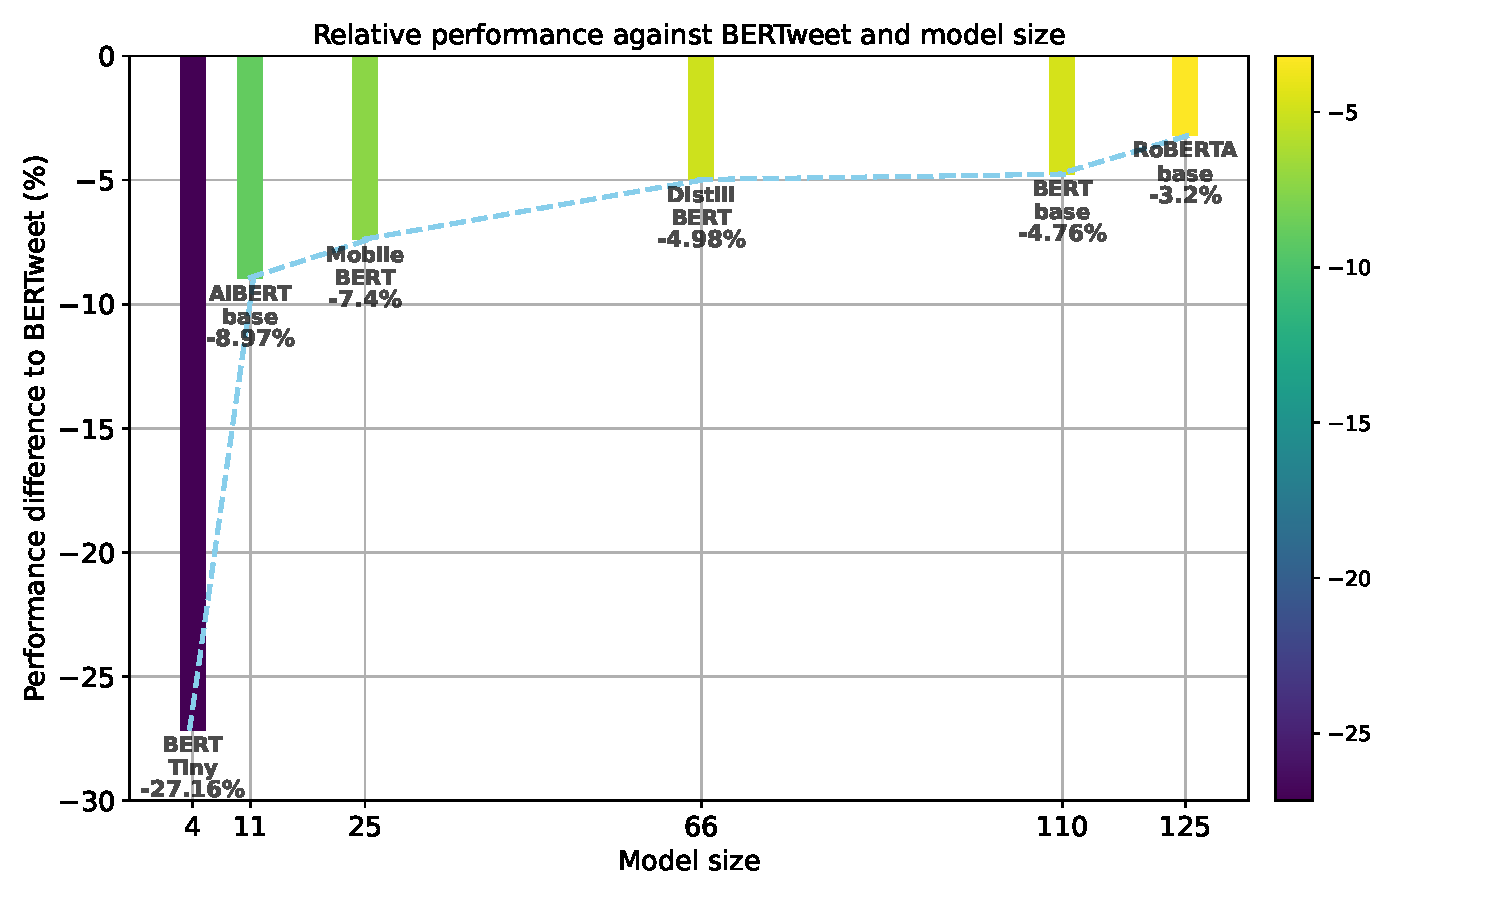
\includegraphics[width=12cm]{figures/model_size_vs_perf.pdf}
    \vspace*{-3mm}
    \caption{Relative performance of models against BERTweet and model sizes based on F1. BERTweet's model size is 110M.}
    \label{fig: model_size_vs_perf}
\end{figure}

% Relative performance table
\begin{table}
    \small
    \centering
    \begin{tabularx}{\textwidth}{|X|c|c|c|c|}
        \hline
        \rowcolor[gray]{0.7}
        \textbf{Model} & \textbf{F1} & \textbf{Model size} & \textbf{Train time} & \textbf{Inference time} \\
        \hline
        \textit{BERTweet}       & \textit{0.908}       & \textit{110M}                & \textit{87.19 s}             & \textit{0.987 s}                 \\
        \hline
        RoBERTa base   & -3.2\%      & +13.6\%             & -4.5\%              & -1.6\%                  \\
        \rowcolor[gray]{0.9}
        BERT base      & -4.8\%      & +0.0\%              & -10.7\%             & +1.2\%                  \\
        DistilBERT     & -5.0\%      & -40.0\%             & -50.7\%             & -43.3\%                 \\
        \rowcolor[gray]{0.9}
        MobileBERT     & -7.4\%      & -77.0\%             & +122.7\%            & +86.4\%                 \\
        ALBERT         & -9.0\%      & -90.0\%             & -40.3\%             & +22.8\%                 \\
        \rowcolor[gray]{0.9}
        BERT Tiny      & -27.1\%     & -96.0\%             & -86.4\%             & -70.2\%                 \\
        \hline
    \end{tabularx}
    \caption{Comparison of key metrics of the models relative to BERTweet.}
    \label{tab: relative_comparison_metrics}
\end{table}

Figure \ref{fig: model_size_vs_perf} displays the relative variance in model performance when compared to BERTweet based on F1, alongside the corresponding model sizes or the number of parameters. Table \ref{tab: relative_comparison_metrics} expands on this by including the relative difference of the models compared to BERTweet in terms of model size, training time and inference time. Notably, ALBERT and MobileBERT exhibit relatively lower performance discrepancies of 8.9\% and 7.4\%, considering the model sizes are significantly smaller by 90\% and 77\% respectively. DistilBERT demonstrates a performance deficit of merely 4.9\%, not far off from BERT base while having a model size lower by 44\%. This could likely be due to the knowledge distillation and compression techniques applied during the pretraining phase, which could be playing a key role in enhancing DistilBERT's predictive capabilities \cite{sanhDistilBERTDistilledVersion2020}.\\

\subsubsection{Analyis of finetuning and inference time}

Next, the time required for inference and training (finetuning) is analysed and shown in Figure \ref{fig: mean_time_taken}. On average, the number of rows for the train, dev and test splits was 2155, 719 and 575. The training and inference were executed on a single NVIDIA RTX A4000 GPU with 16GB VRAM. BERT Tiny as expected has the lowest mean training and inference time. It is lower by over 85\% and 70\% for training and inference respectively as shown in Table \ref{tab: relative_comparison_metrics} when compared to BERTweet. DistilBERT follows next with lower train and inference times by 51\% and 43\%. For ALBERT the train time is lower than BERTweet by 40\%, while the inference time is slightly higher than BERT base. The architecture of ALBERT is designed such that the training time is reduced there is a low memory footprint and it is not expected to significantly lower the inference time. MobileBERT shows very high training and inference times and is 123\% and 86\% higher than BERTweet.
% training and inference time bar chart
\begin{figure}[htbp]
    \centering
    \captionsetup{font=small}
    \begin{subfigure}{0.49\textwidth}
        \centering
        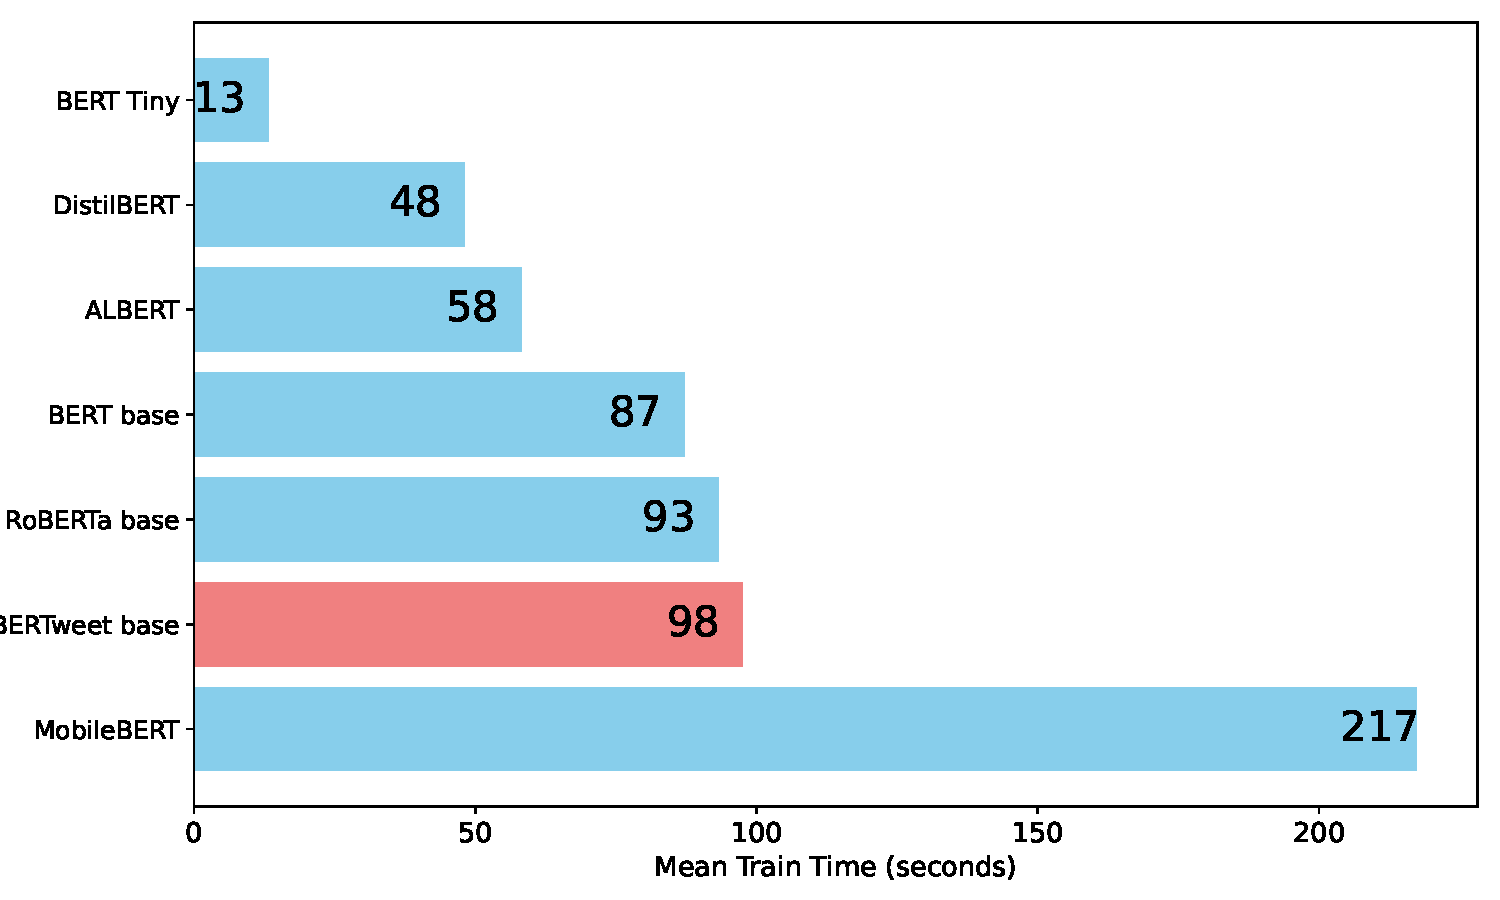
\includegraphics[width=\linewidth]{figures/mean_train_time.pdf}
        \caption{Mean training time.}
        \label{fig: mean_train_time}
    \end{subfigure}
    \hfill
    \begin{subfigure}{0.49\textwidth}
        \centering
        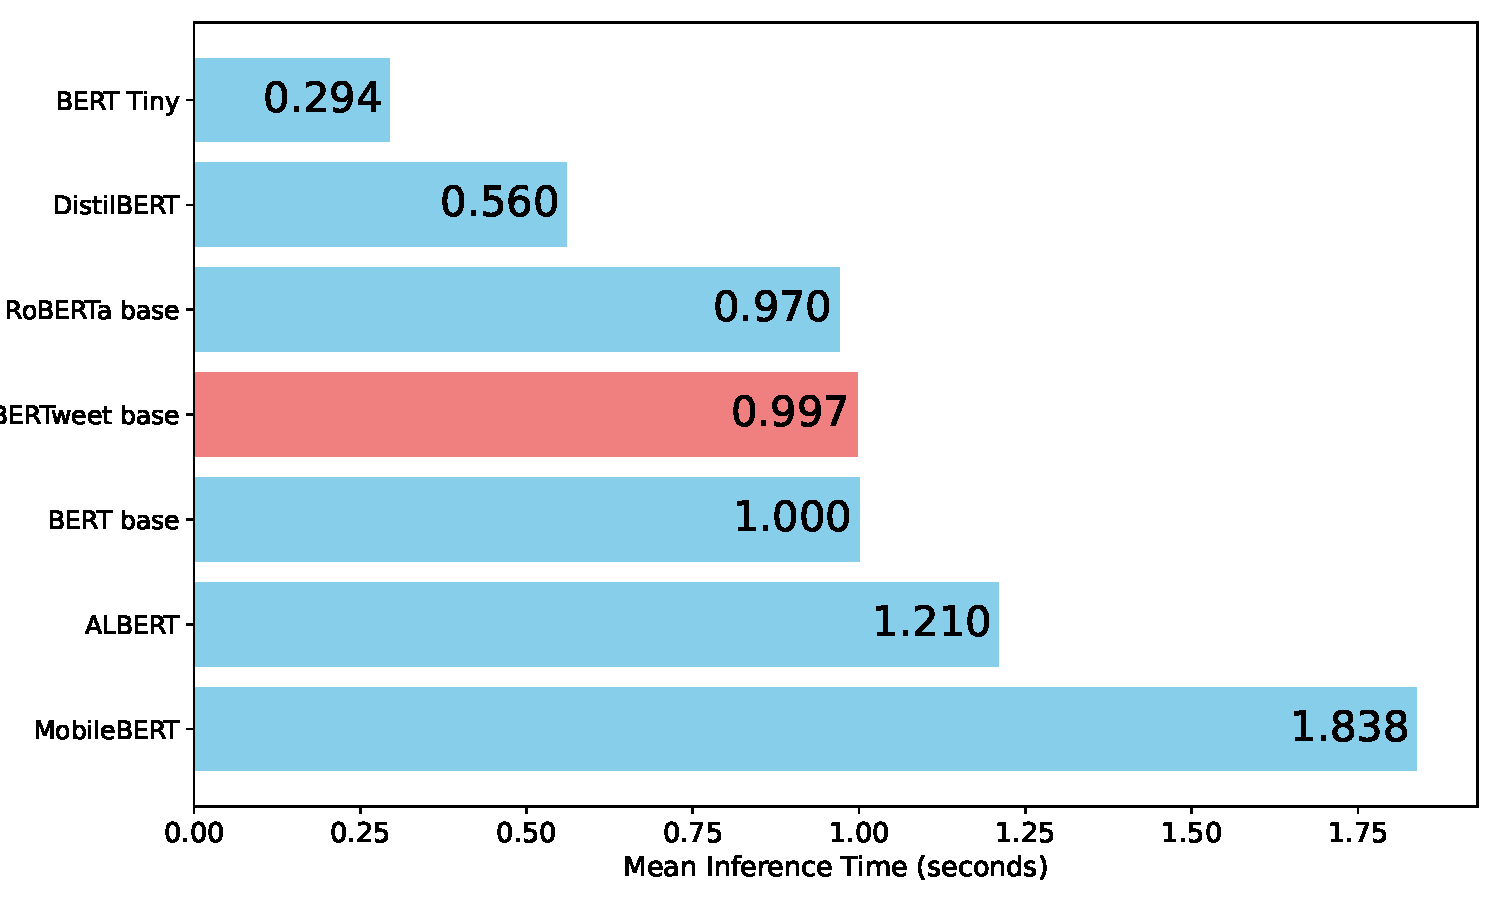
\includegraphics[width=\linewidth]{figures/mean_inference_time.pdf}
        \caption{Mean inference time}
        \label{fig: mean_inf_time}
    \end{subfigure}
    \caption{Mean time taken (in seconds) for finetuning and inference during experiments set 1. BERTweet with the best predictive model is highlighted in red.}
    \label{fig: mean_time_taken}
\end{figure}

\subsection{Deep-dive into the results}
To comprehend where the models are misclassifying, deep-dive analysis is carried out on the performance of select models. The overall best-performing model, BERTweet Base, the best-performing lightweight model, DistilBERT and the worst-performing model, BERT Tiny are chosen for this exercise. The confusion matrix, sample misclassified tweets and Mathews Correlation Coefficient (MCC) will be analysed for them. The confusion matrix and MCC are based on the mean values from the 6 runs of inference carried out.\\
% Test loss table
\begin{table}[ht]
    \centering
    \begin{tabularx}{\textwidth}{|X|X|X|X|}
        \hline
        \rowcolor[gray]{0.7}
        \textbf{Test Run} & \textbf{BERTweet Base} & \textbf{DistilBERT} & \textbf{BERT Tiny} \\
        \hline
        1                 & 0.21701                & 0.22481             & 0.49180            \\
        \rowcolor[gray]{0.9}
        2                 & 0.20056                & 0.24783             & 0.50118            \\
        3                 & 0.23015                & 0.26190             & 0.48807            \\
        \rowcolor[gray]{0.9}
        4                 & 0.23572                & 0.25394             & 0.48178            \\
        5                 & 0.25255                & 0.30100             & 0.53076            \\
        \rowcolor[gray]{0.9}
        6                 & 0.17506                & 0.26712             & 0.48810            \\
        \hline
    \end{tabularx}
    \caption{Test loss from the inference phase for the 6 outer loop iterations for the 3 selected models.}
    \label{tab: test_loss}
\end{table}

% Deep dive confusion matrices and line graphs
\begin{figure}[!ht]
    \small
    \centering
    \begin{subfigure}{0.45\linewidth}
        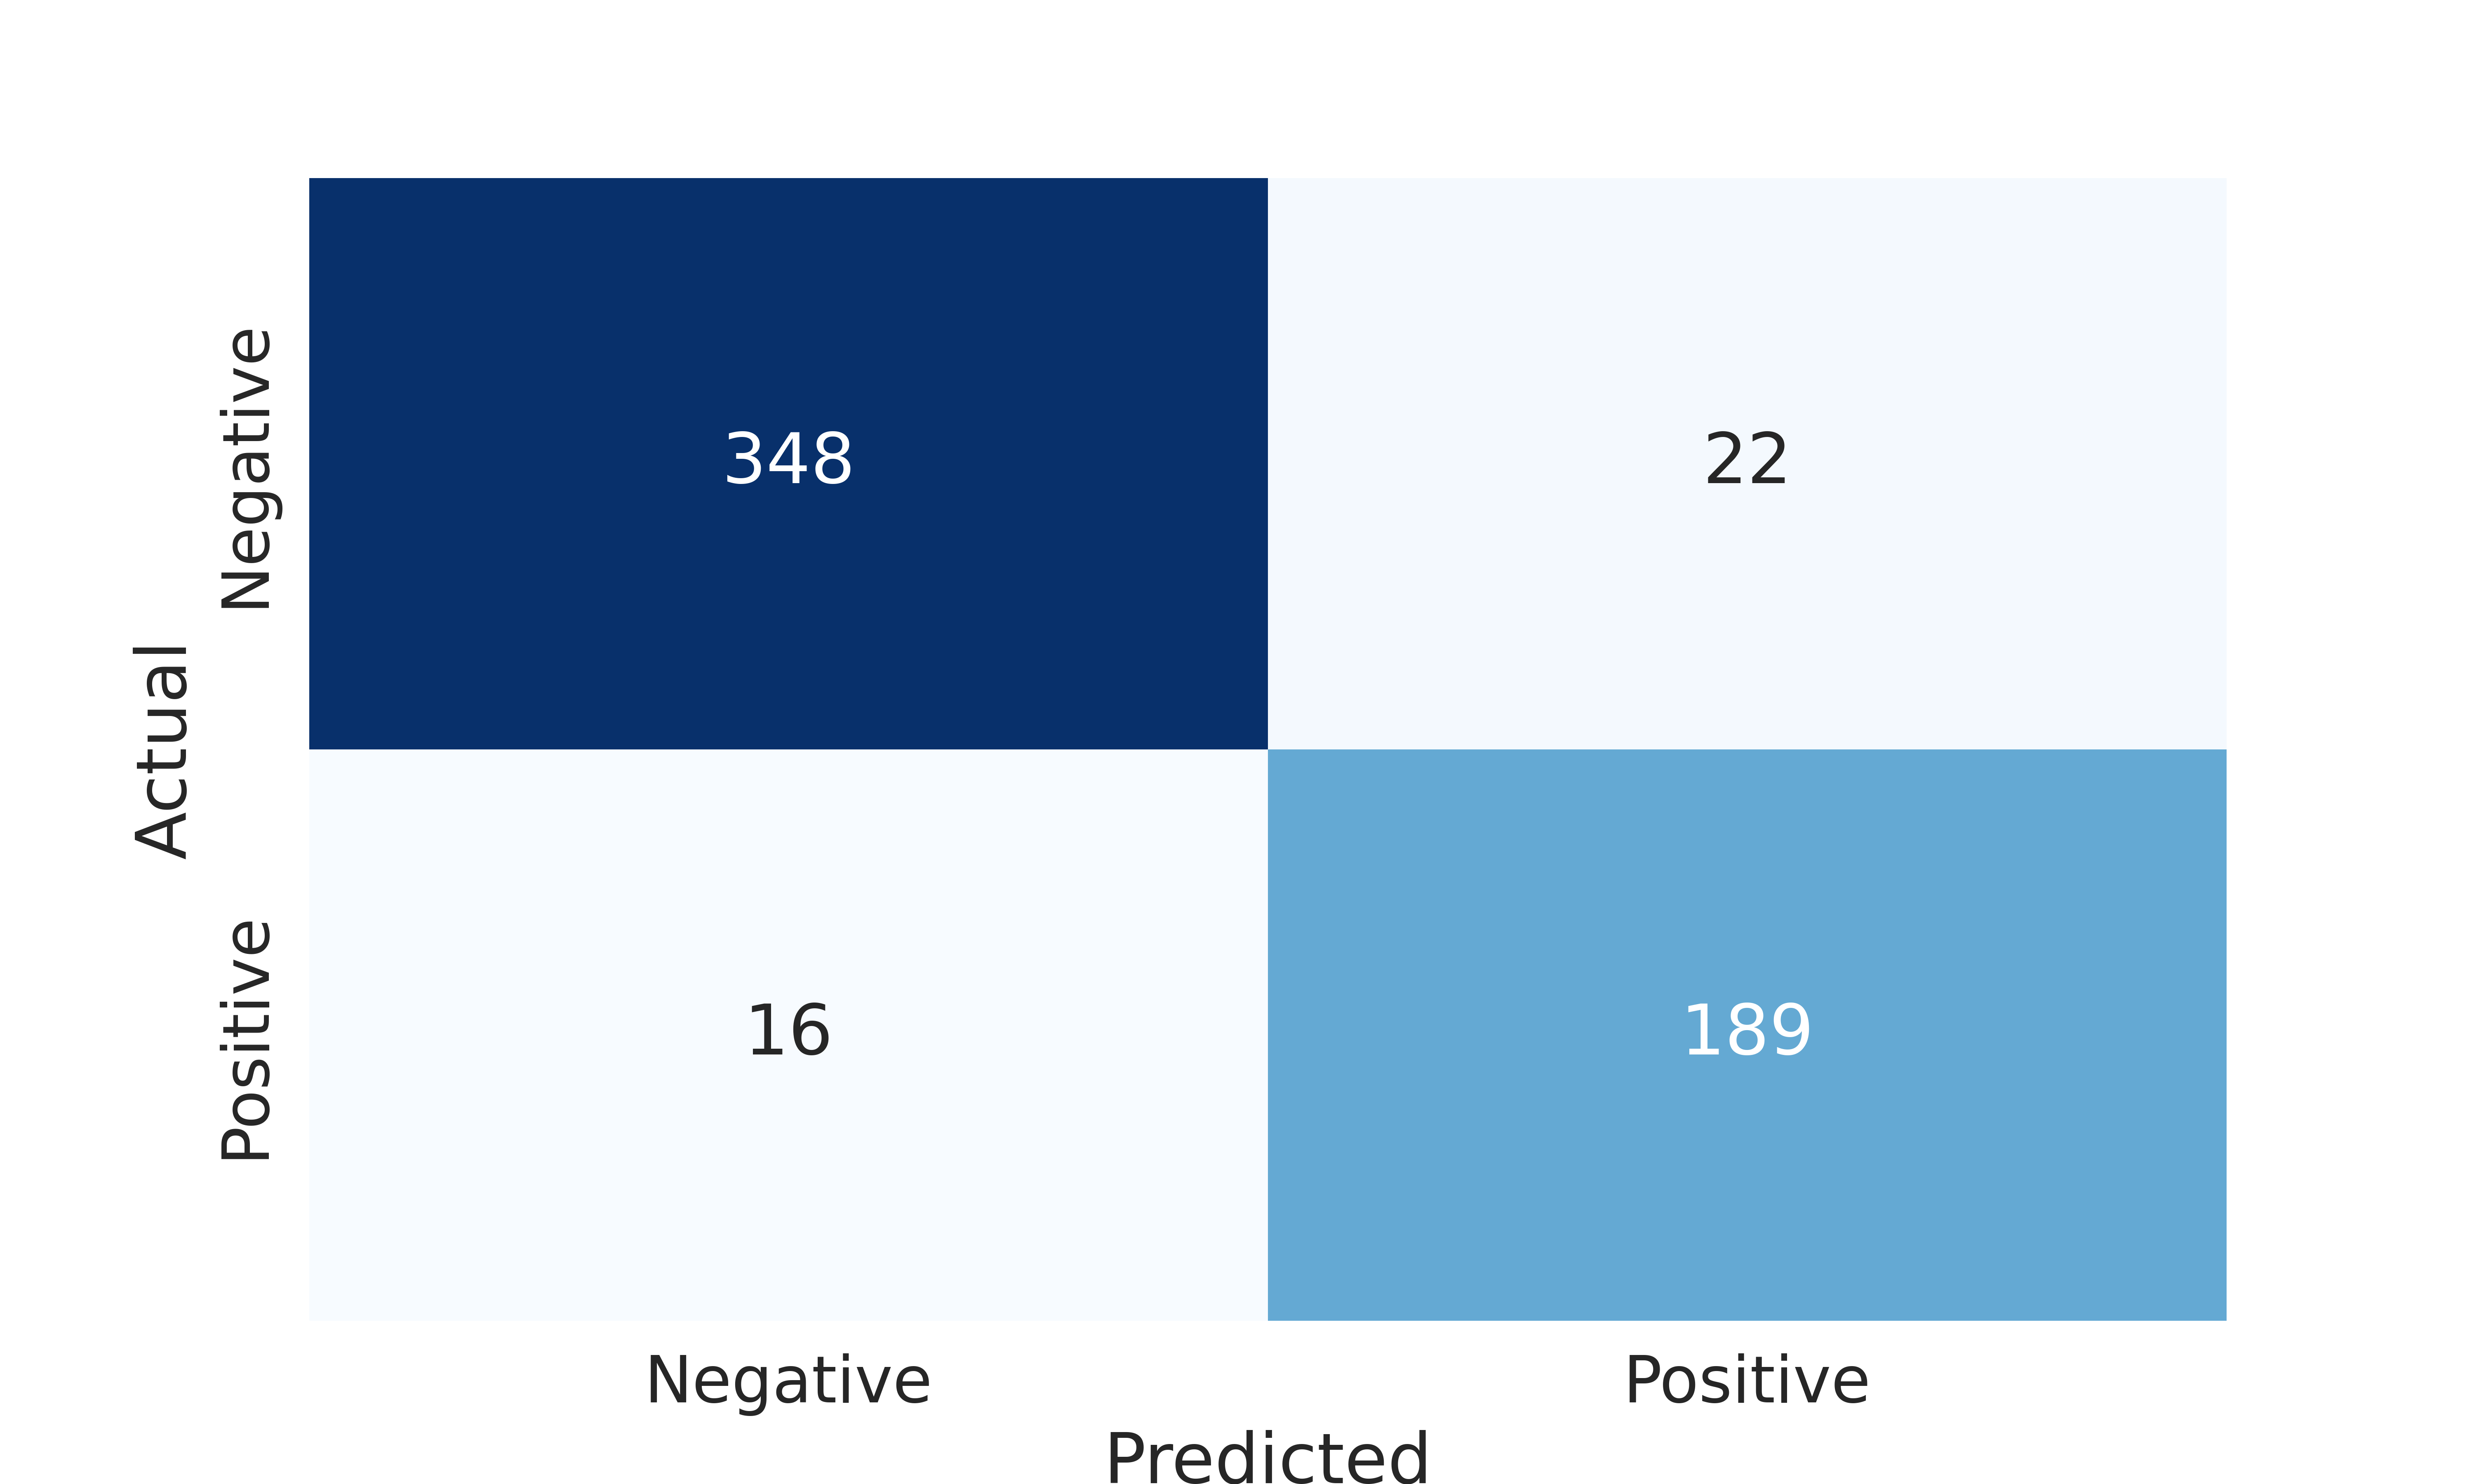
\includegraphics[width=\linewidth]{figures/confusion_bertweet.png}
        \caption{BERTweet - Confusion Matrix}
    \end{subfigure}
    \hfil
    \begin{subfigure}{0.45\linewidth}
        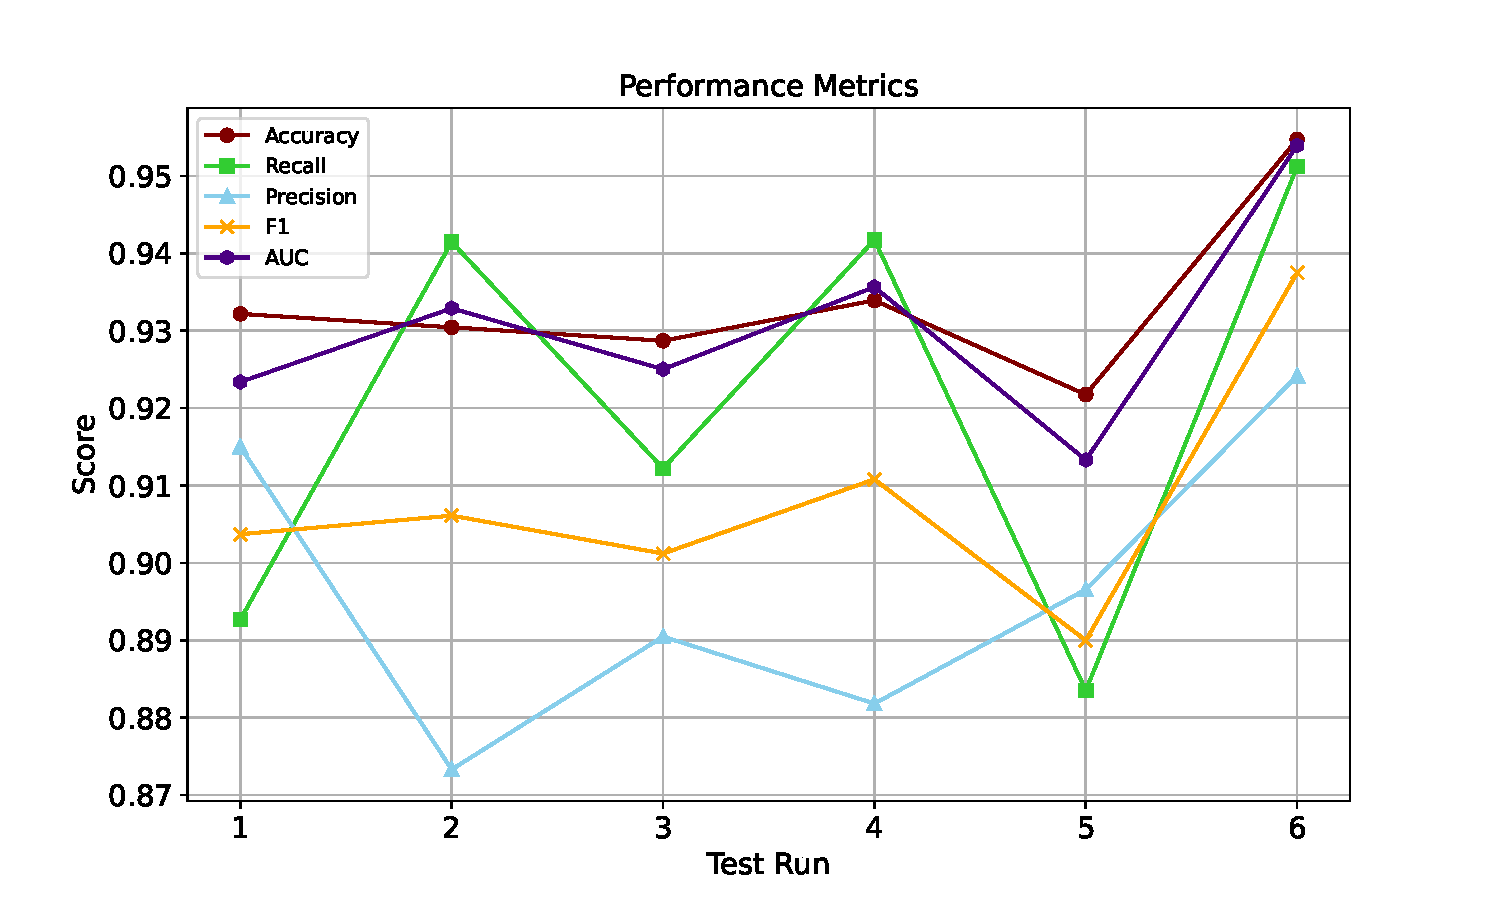
\includegraphics[width=\linewidth]{figures/metrics_line_bertweet.pdf}
        \caption{BERTweet - Performance Metrics}
    \end{subfigure}

    \begin{subfigure}{0.45\linewidth}
        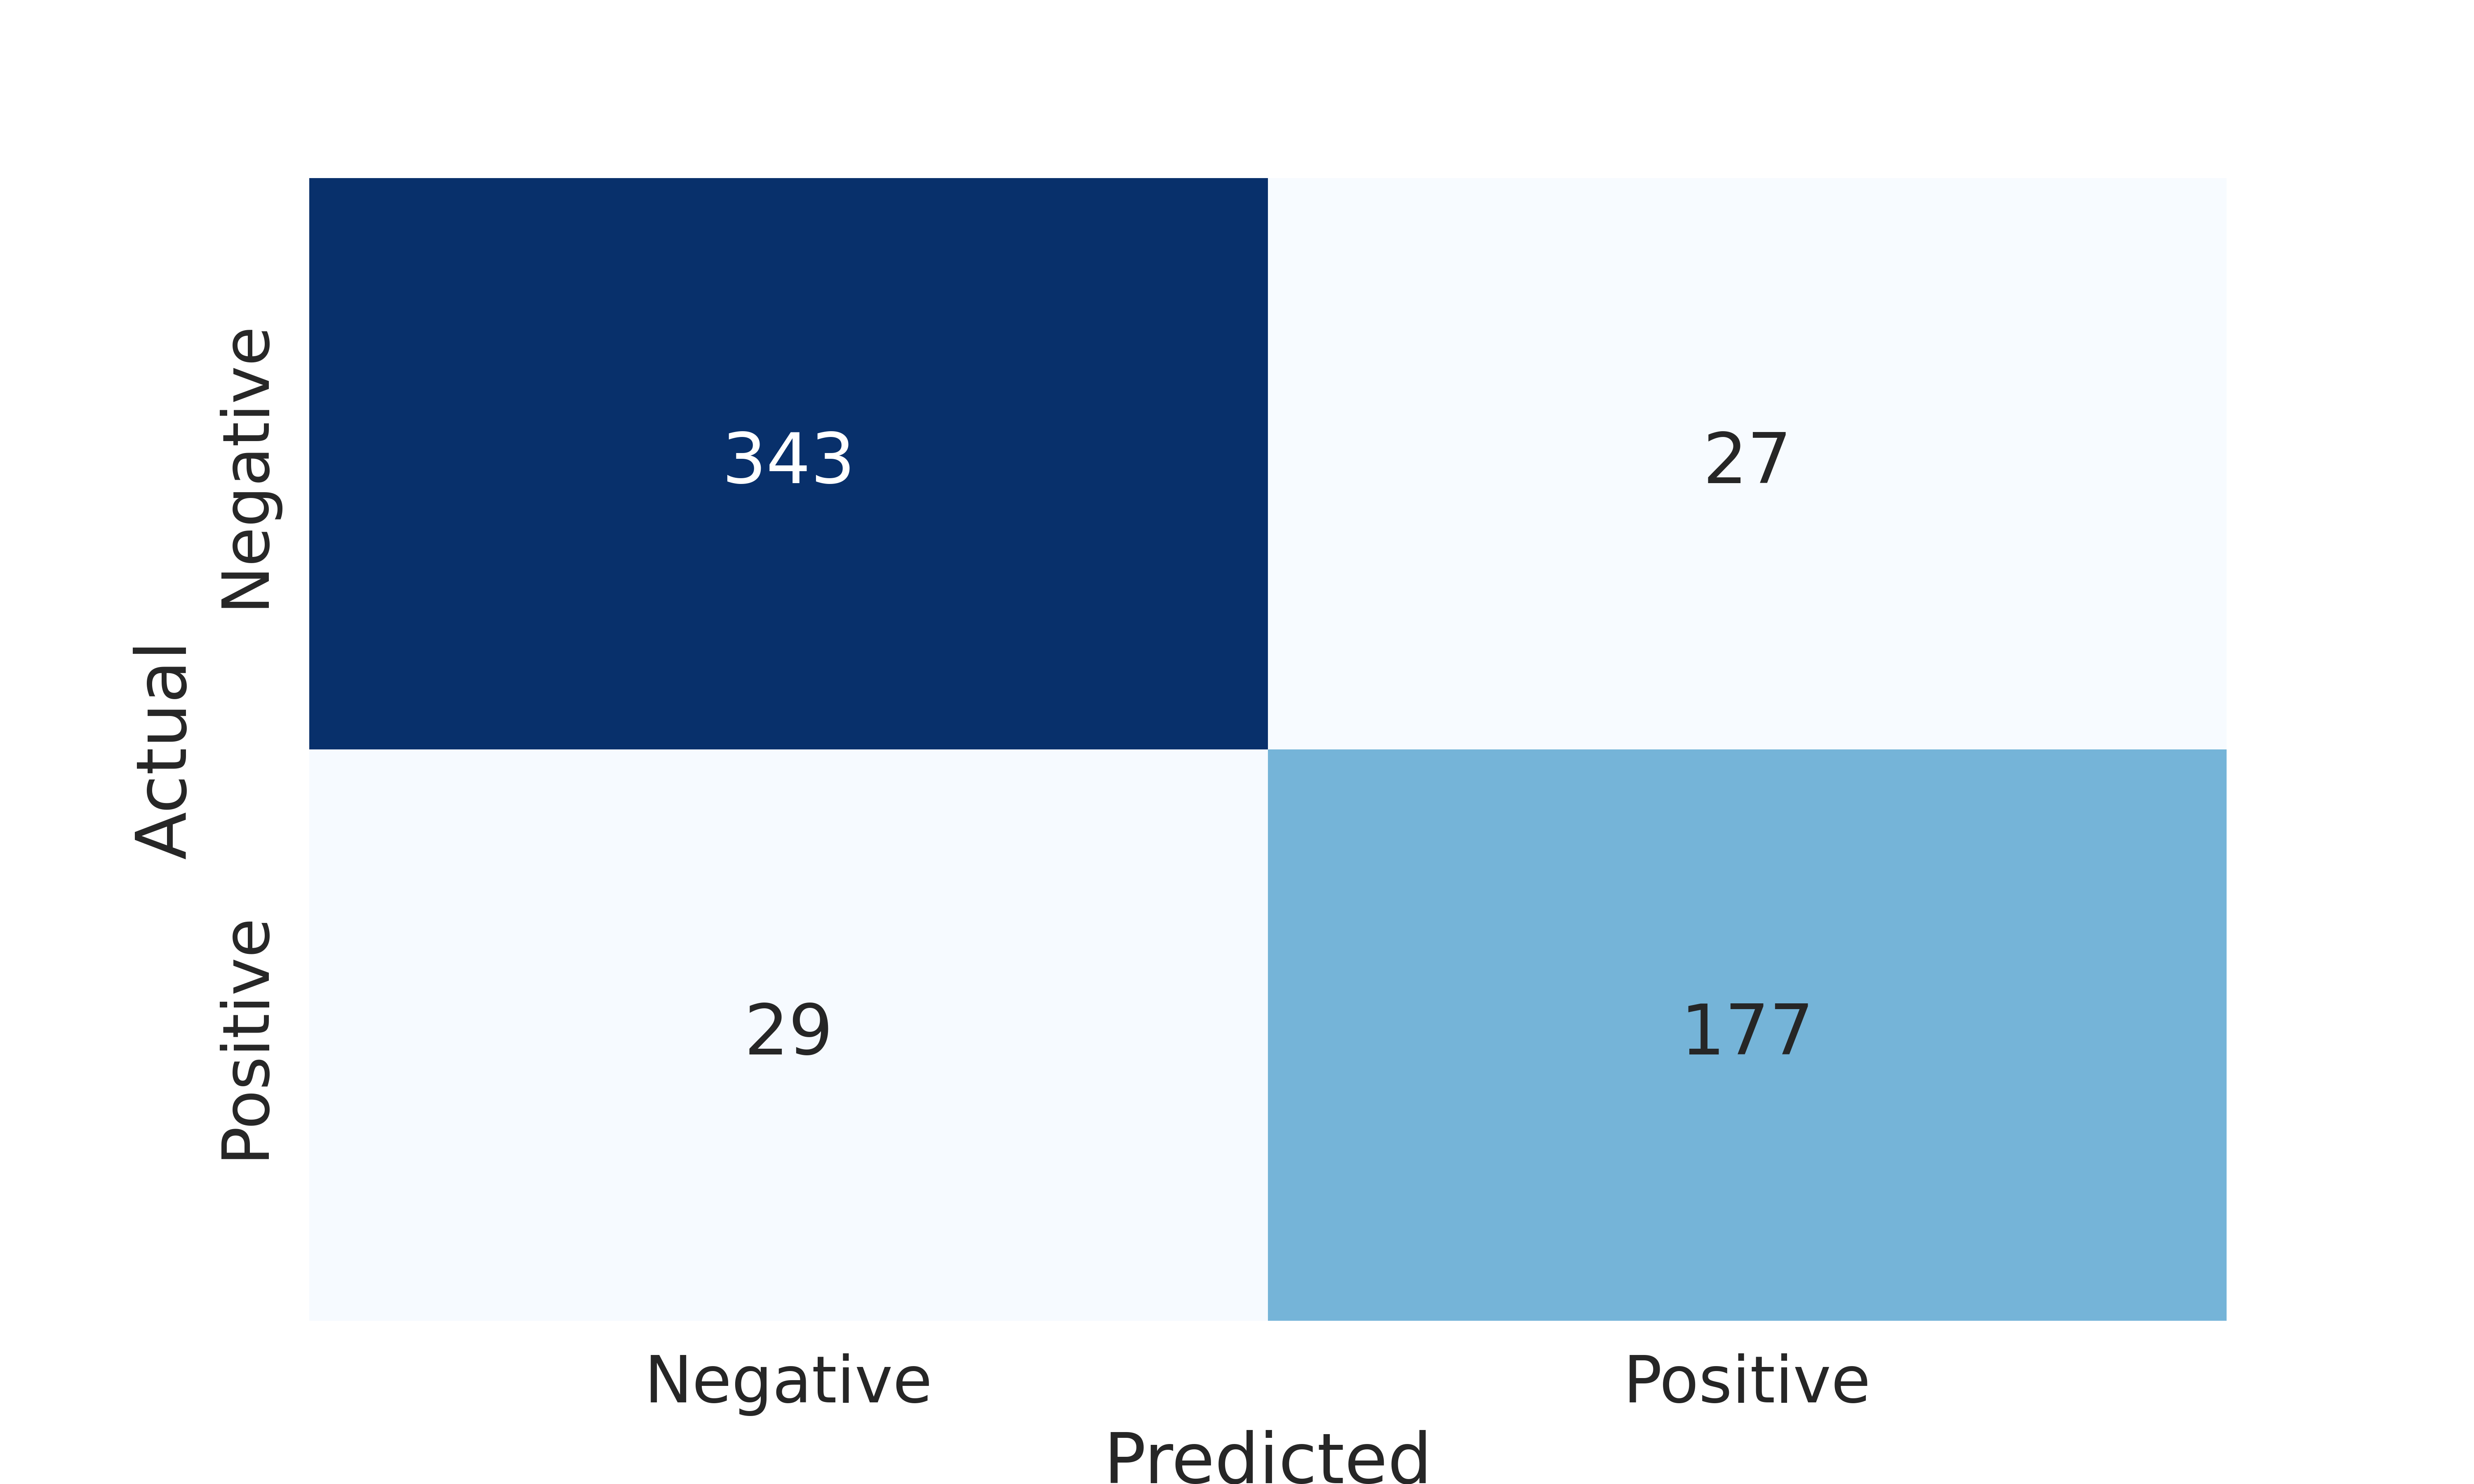
\includegraphics[width=\linewidth]{figures/confusion_distilbert.png}
        \caption{DistilBERT - Confusion Matrix}
    \end{subfigure}
    \hfil
    \begin{subfigure}{0.45\linewidth}
        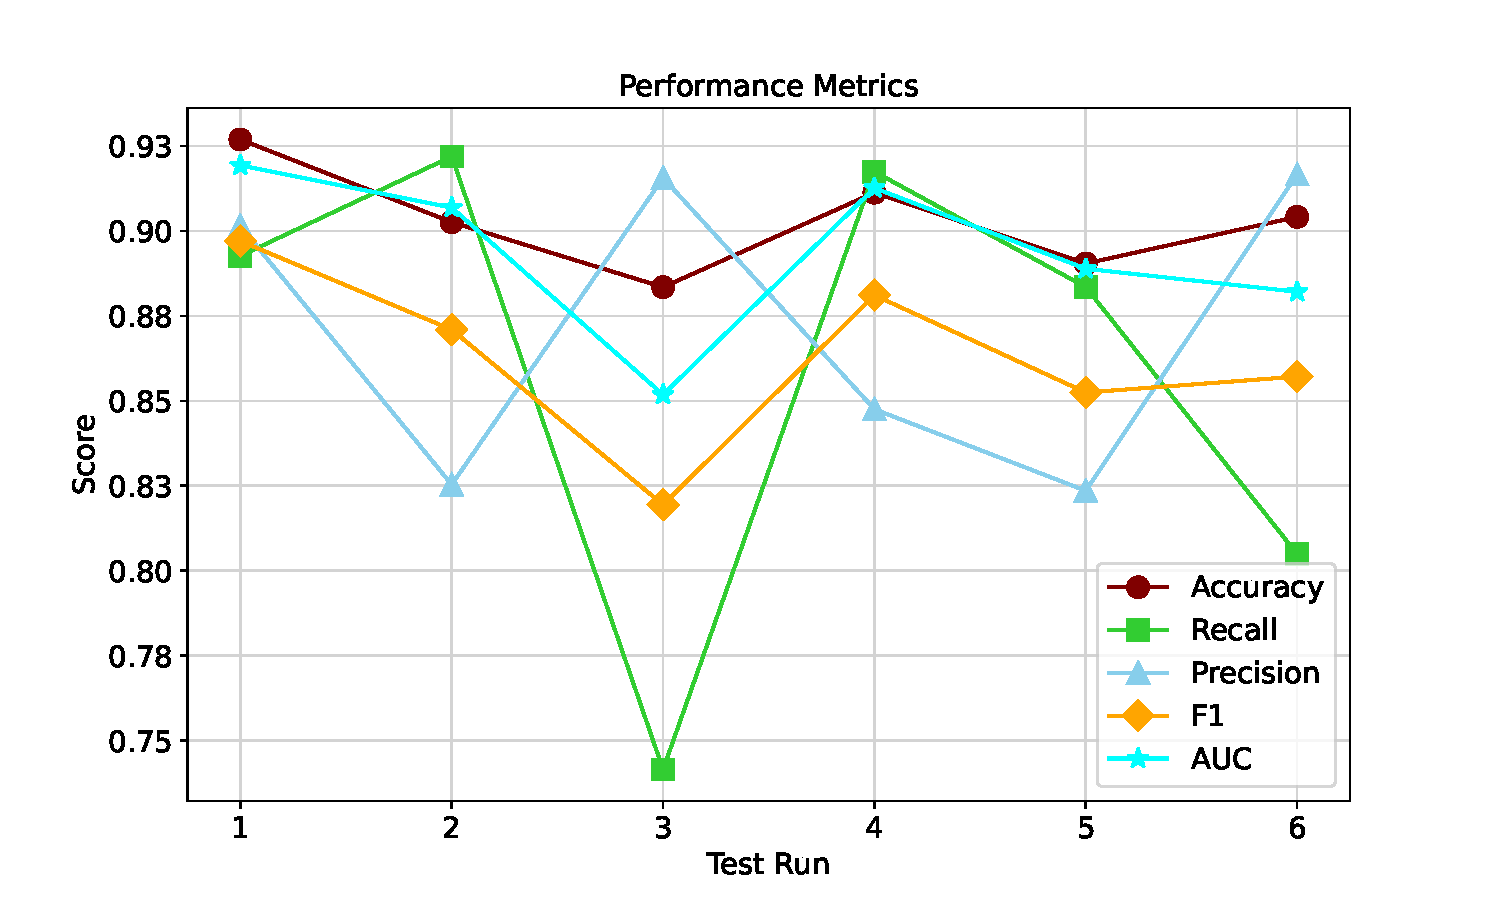
\includegraphics[width=\linewidth]{figures/metrics_line_distilbert.pdf}
        \caption{DistilBERT - Performance Metrics}
    \end{subfigure}

    \begin{subfigure}{0.45\linewidth}
        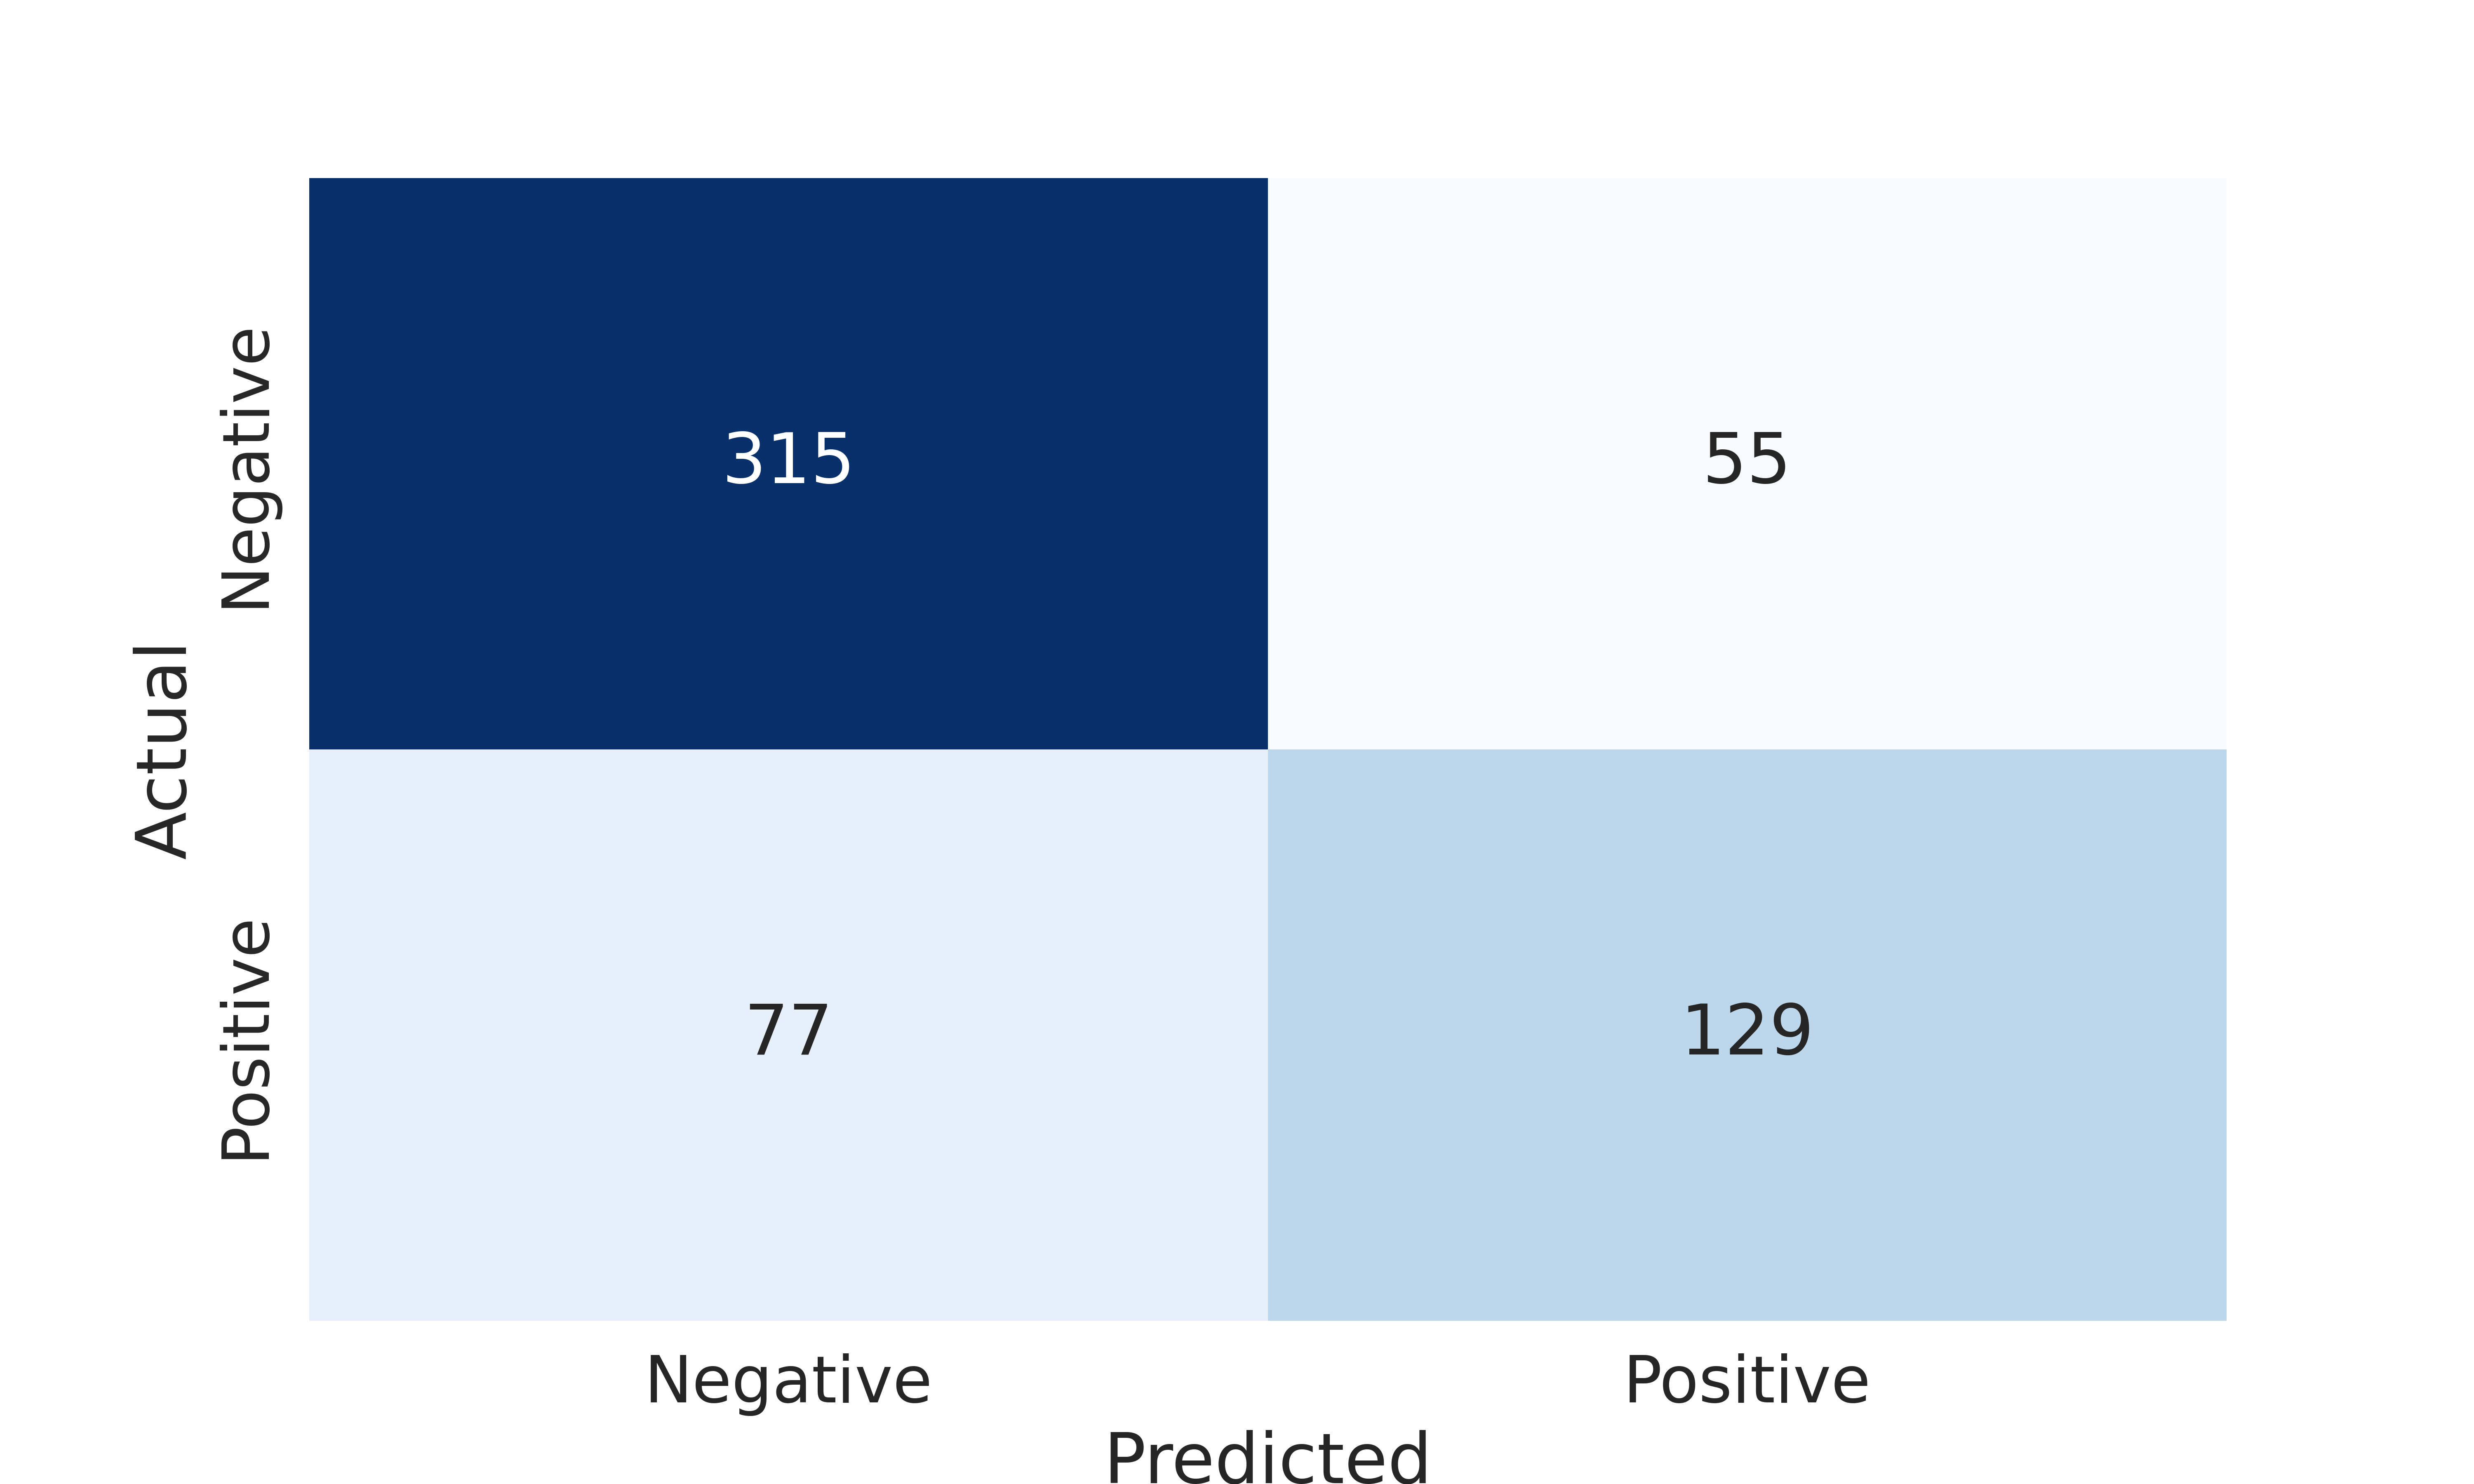
\includegraphics[width=\linewidth]{figures/confusion_berttiny.png}
        \caption{BERT Tiny - Confusion Matrix}
    \end{subfigure}
    \hfil
    \begin{subfigure}{0.45\linewidth}
        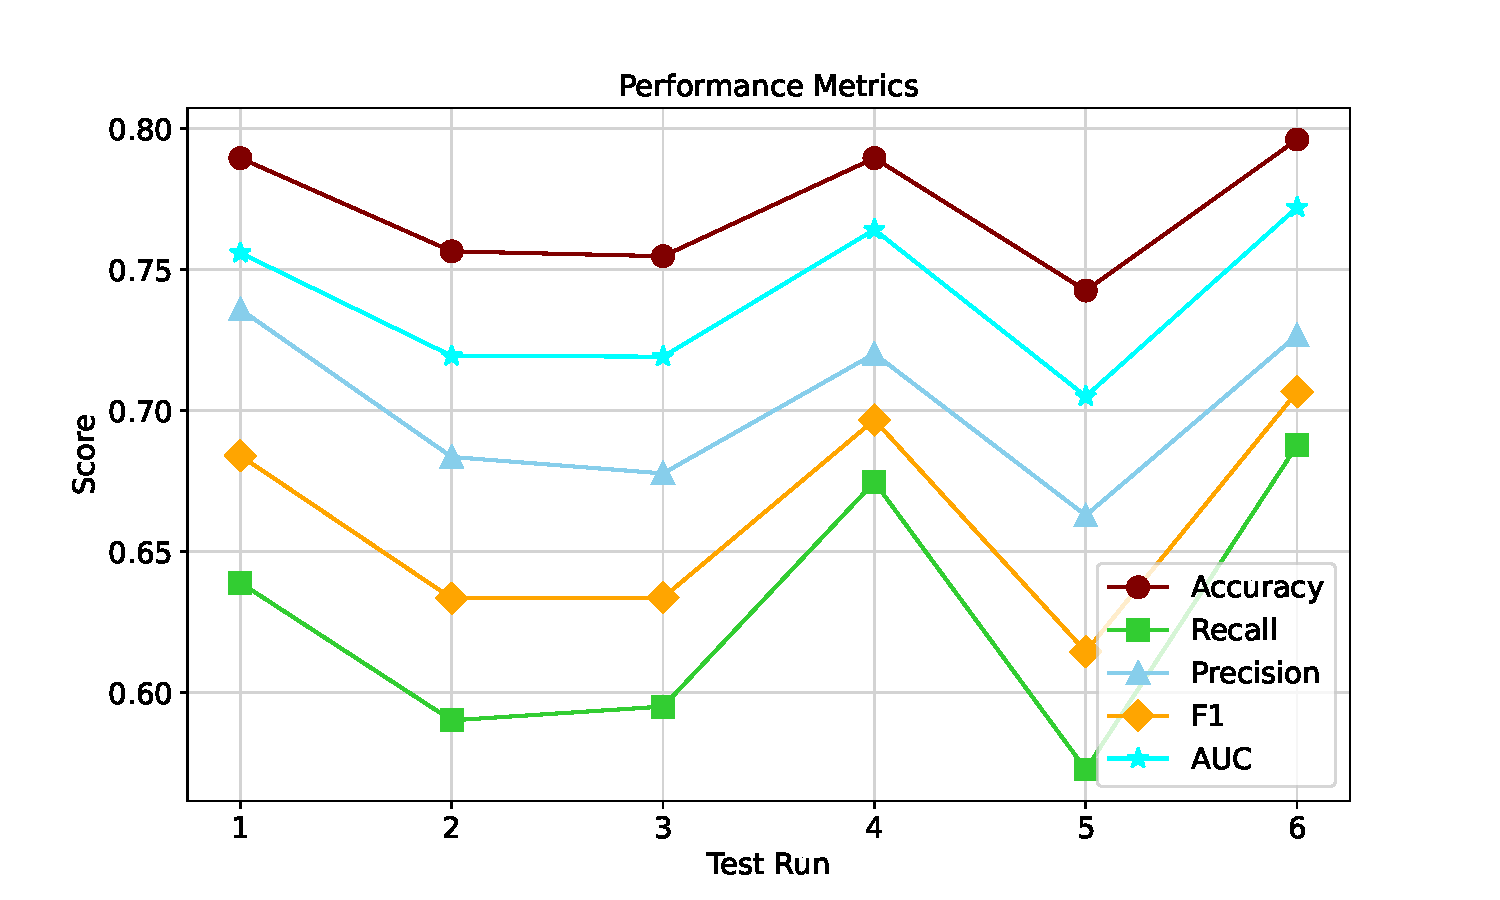
\includegraphics[width=\linewidth]{figures/metrics_line_berrttiny.pdf}
        \caption{BERT Tiny - Performance Metrics}
    \end{subfigure}
    \caption{Confusion matrix and performance metrics for the 3 selected models from the inference phase. The confusion matrix is based on the mean of values from the 6 outer loop iterations and the grid can be read from left to right as true negative, false positive, false negative and true positive.}
    \label{fig: deep_dive_results}
\end{figure}

The test losses for the 6 runs are given in Table \ref{tab: test_loss} while the graphs for the performance scores from inference are illustrated in Figure \ref{fig: deep_dive_results}. As expected, the test loss is lower for most the of 6 runs for BERTweet Base compared to the other two models. We find DistilBERT Base having losses that are closer to BERT Base in 2 runs but otherwise are generally higher. There is a considerable difference for BERT Tiny which reflects in the predictive performance scores discussed earlier. \\

Referring to the metrics in Figure \ref{fig: deep_dive_results}, BERT Tiny exhibits a pattern that differs from the other 2 models. Based on the correct and incorrect classifications for all the inference executions (detailed in \ref{sec: conf_matrix_test_runs}), it appears that within each test run, the change in the misclassified complaint and non-complaint tweets move in the same direction. Another point to note is that BERTweet and DistilBERT seem to have relatively high fluctuations in recall and precision, likely due to inherent variations in the data splits from the cross-folds for each run. Considering the classes are imbalanced the ROC AUC score is also analysed. While BERTweet shows the best discrimination ability among the 3 models based on the AUC score, it also has the least amount of variability with a standard deviation of 0.01. DistilBERT has higher \\

Figure \ref{fig: deep_dive_results} also shows the confusion matrices for the 3 models based on the mean of the classifications from the 6 test runs. The ratio of accurately categorized non-complaint tweets (true negatives) to complaint tweets (true positives) is comparable between BERTweet and DistilBERT, but it's lower for BERT Tiny. All models appear to face greater challenges in accurately classifying complaint tweets compared to non-complaint tweets, although BERTWeet has the best recall scores overall. Even though there is an inherent class imbalance in the dataset, the confusion matrix and the metrics presented still offer valuable insights into the predictive capabilities of the models\\

% error analysis tweets
\begin{table}
    \small
    \centering
    \begin{tblr}{
        width = \linewidth,
        colspec = {Q[35]Q[908]},
        row{1} = {Nobel,c},
        row{2} = {c},
        row{5} = {Mercury},
        row{6} = {Mercury},
        row{7} = {c},
        row{10} = {Mercury},
        row{11} = {Mercury},
        row{12} = {c},
        row{15} = {Mercury},
        row{16} = {Mercury},
        cell{2}{1} = {c=2}{0.943\linewidth},
        cell{7}{1} = {c=2}{0.943\linewidth},
        cell{12}{1} = {c=2}{0.943\linewidth},
        hlines,
        vlines,
        }
        \textbf{No.}        & \textbf{Tweet}\\
        \textbf{BERTweet}   & \\
        1                   & do potato based products belong in sandwiches ?\\
        2                   & worst *\\
        3                   & i had entered in giveway contest for oneplus 5t lava . so waiting for the result\\
        4                   & i just checked again and i'm not having the same issues i had earlier . thanks for the help\\
        \textbf{DistilBERT} & \\
        5                   & hey guys , i love this product featured on user today but don't see a price ? help a girl out ?\\
        6                   & is this really what you call a large milkshake <user> <url>\\
        7                   & shout out to the social media team <user> <user> whilst i get the frustration , there's never a time people should be insulting or rude when tweeting . these good people responding are employee's just tyring to help . \#heathrowairport \#heathrow \#britishairways \\
        8                   & no , see screenshot . it's the app . i got it straight off the playstore on android .\\
        \textbf{BERT Tiny}  &\\
        9                   & whyyyy is your wifi so slow <user> ?\\
        10                  & my 2nd visit to kfc chadwell heath after the last fiasco . this time they had no gravy or corn  amp ; forgot my chips \#fail\\
        11                  & is it possible to integrate my medium account on my personal website with your api ?\\
        12                  & thanks for your response . what is the twitter handle for your care centre in delhi , india ?
    \end{tblr}
    \caption{Sample tweets which have been misclassified by the 3 selected models. Tweets in the \colorbox{Mercury}{lighter shade of grey} are misclassified as complaints while the rest are misclassified as not complaints.}
    \label{tab: error_tweets}
\end{table}
 
Next, an error analysis is conducted on the tweets that were misclassified. Sample tweets that were inaccurately classified by the three models are presented in Table \ref{tab: error_tweets}. Examining tweets that were wrongly labelled as non-complaints by BERTweet and DistilBERT, several observations are discussed. The models seem to have challenges in identifying sarcasm within a constrained linguistic context (example 1), the presence of very concise text (example 2), the combination of mild expressions of dissatisfaction with questions (example 5), and the usage of rhetorical questions (example 6). Notably, BERT Tiny struggles even when tweets exhibit multiple indicators of being complaints, as seen in examples 9 and 10. Regarding tweets that were erroneously classified as complaints, instances include tweets containing words commonly associated with grievances, like 'waiting' and 'issue' (examples 3 and 4), as well as tweets that narrate negative experiences rather than expressing complaints (example 7). Additionally, instances arise where the text represents an intermediate segment of a conversation (example 8). BERT Tiny appears to get confused when encountering text containing questions which do not no hint of complaining and are about mundane topics  (examples 11 and 12).

\section{Experiment set 2 results: Cross-domain results}
% Cross domain results table
\begin{table}
    \centering
    \resizebox{\linewidth}{!}{%
        \begin{tblr}{
            row{odd} = {Mercury},
            row{1} = {Nobel},
            cell{2}{2} = {c},
            cell{2}{3} = {c},
            cell{2}{4} = {c},
            cell{2}{5} = {c},
            cell{2}{6} = {c},
            cell{2}{7} = {c},
            cell{2}{8} = {c},
            cell{2}{9} = {c},
            cell{2}{10} = {c},
            cell{3}{2} = {c},
            cell{3}{3} = {c},
            cell{3}{4} = {c},
            cell{3}{5} = {c},
            cell{3}{6} = {c},
            cell{3}{7} = {c},
            cell{3}{8} = {c},
            cell{3}{9} = {c},
            cell{3}{10} = {c},
            cell{4}{2} = {c},
            cell{4}{3} = {c},
            cell{4}{4} = {c},
            cell{4}{5} = {c},
            cell{4}{6} = {c},
            cell{4}{7} = {c},
            cell{4}{8} = {c},
            cell{4}{9} = {c},
            cell{4}{10} = {c},
            cell{5}{2} = {c},
            cell{5}{3} = {c},
            cell{5}{4} = {c},
            cell{5}{5} = {c},
            cell{5}{6} = {c},
            cell{5}{7} = {c},
            cell{5}{8} = {c},
            cell{5}{9} = {c},
            cell{5}{10} = {c},
            cell{6}{2} = {c},
            cell{6}{3} = {c},
            cell{6}{4} = {c},
            cell{6}{5} = {c},
            cell{6}{6} = {c},
            cell{6}{7} = {c},
            cell{6}{8} = {c},
            cell{6}{9} = {c},
            cell{6}{10} = {c},
            cell{7}{2} = {c},
            cell{7}{3} = {c},
            cell{7}{4} = {c},
            cell{7}{5} = {c},
            cell{7}{6} = {c},
            cell{7}{7} = {c},
            cell{7}{8} = {c},
            cell{7}{9} = {c},
            cell{7}{10} = {c},
            cell{8}{2} = {c},
            cell{8}{3} = {c},
            cell{8}{4} = {c},
            cell{8}{5} = {c},
            cell{8}{6} = {c},
            cell{8}{7} = {c},
            cell{8}{8} = {c},
            cell{8}{9} = {c},
            cell{8}{10} = {c},
            cell{9}{2} = {c},
            cell{9}{3} = {c},
            cell{9}{4} = {c},
            cell{9}{5} = {c},
            cell{9}{6} = {c},
            cell{9}{7} = {c},
            cell{9}{8} = {c},
            cell{9}{9} = {c},
            cell{9}{10} = {c},
            cell{10}{2} = {c},
            cell{10}{3} = {c},
            cell{10}{4} = {c},
            cell{10}{5} = {c},
            cell{10}{6} = {c},
            cell{10}{7} = {c},
            cell{10}{8} = {c},
            cell{10}{9} = {c},
            cell{10}{10} = {c},
            cell{11}{2} = {c},
            cell{11}{3} = {c},
            cell{11}{4} = {c},
            cell{11}{5} = {c},
            cell{11}{6} = {c},
            cell{11}{7} = {c},
            cell{11}{8} = {c},
            cell{11}{9} = {c},
            cell{11}{10} = {c},
            vlines,
            hline{1-2,11-12} = {-}{},
                    hline{3} = {2-10}{white},
                }
            \diagbox{\textbf{Train}}{\textbf{Test}} & \textbf{Food}  & \textbf{Appr. } & \textbf{Cars } & \textbf{Retail } & \textbf{Srvcs. } & \textbf{Softw. } & \textbf{Trans. } & \textbf{Elect. } & \textbf{Other } \\
            \textbf{Food}                           & -              & 0.515           & 0.522          & 0.528            & 0.532            & \textbf{0.534}   & 0.517            & 0.529            & 0.510           \\
            \textbf{Appr.}                          & \textbf{0.854} & -               & 0.775          & 0.828            & 0.807            & 0.852            & 0.801            & 0.795            & 0.830           \\
            \textbf{Cars}                           & 0.500          & 0.500           & -              & 0.500            & 0.500            & 0.500            & 0.500            & 0.500            & 0.500           \\
            \textbf{Retail}                         & \textbf{0.798} & 0.706           & 0.715          & -                & 0.698            & 0.752            & 0.698            & 0.701            & 0.666           \\
            \textbf{Srvcs.}                         & 0.820          & 0.829           & 0.781          & 0.812            & -                & 0.834            & 0.802            & 0.824            & \textbf{0.885}  \\
            \textbf{Softw.}                         & \textbf{0.789} & 0.761           & 0.747          & 0.786            & 0.738            & -                & 0.736            & 0.757            & 0.748           \\
            \textbf{Trans.}                         & 0.853          & 0.813           & 0.800          & 0.833            & 0.807            & 0.840            & -                & 0.777            & \textbf{0.871}  \\
            \textbf{Elect.}                         & 0.825          & 0.834           & 0.813          & 0.847            & 0.825            & \textbf{0.853}   & 0.79             & -                & 0.843           \\
            \textbf{Other}                          & 0.500          & 0.500           & 0.500          & 0.500            & 0.500            & 0.500            & 0.500            & 0.500            & -               \\
            \textbf{All}                            & 0.870          & 0.856           & 0.837          & 0.879            & 0.851            & 0.882            & 0.824            & 0.838            & \textbf{0.908}
        \end{tblr}
    }
    \caption{ROC-AUC scores for the cross-domain experiments. The rows hold the domain used for finetuning while the columns represent the domains used for testing. The last row are the scores where the full data except the corresponding test domain was used for finetuning. Best scores where applicable are highlighted in bold.}
    \label{tab: cross_domain_results}
\end{table}

% cross domain heatmap
\begin{figure}[htb]
    \centering
    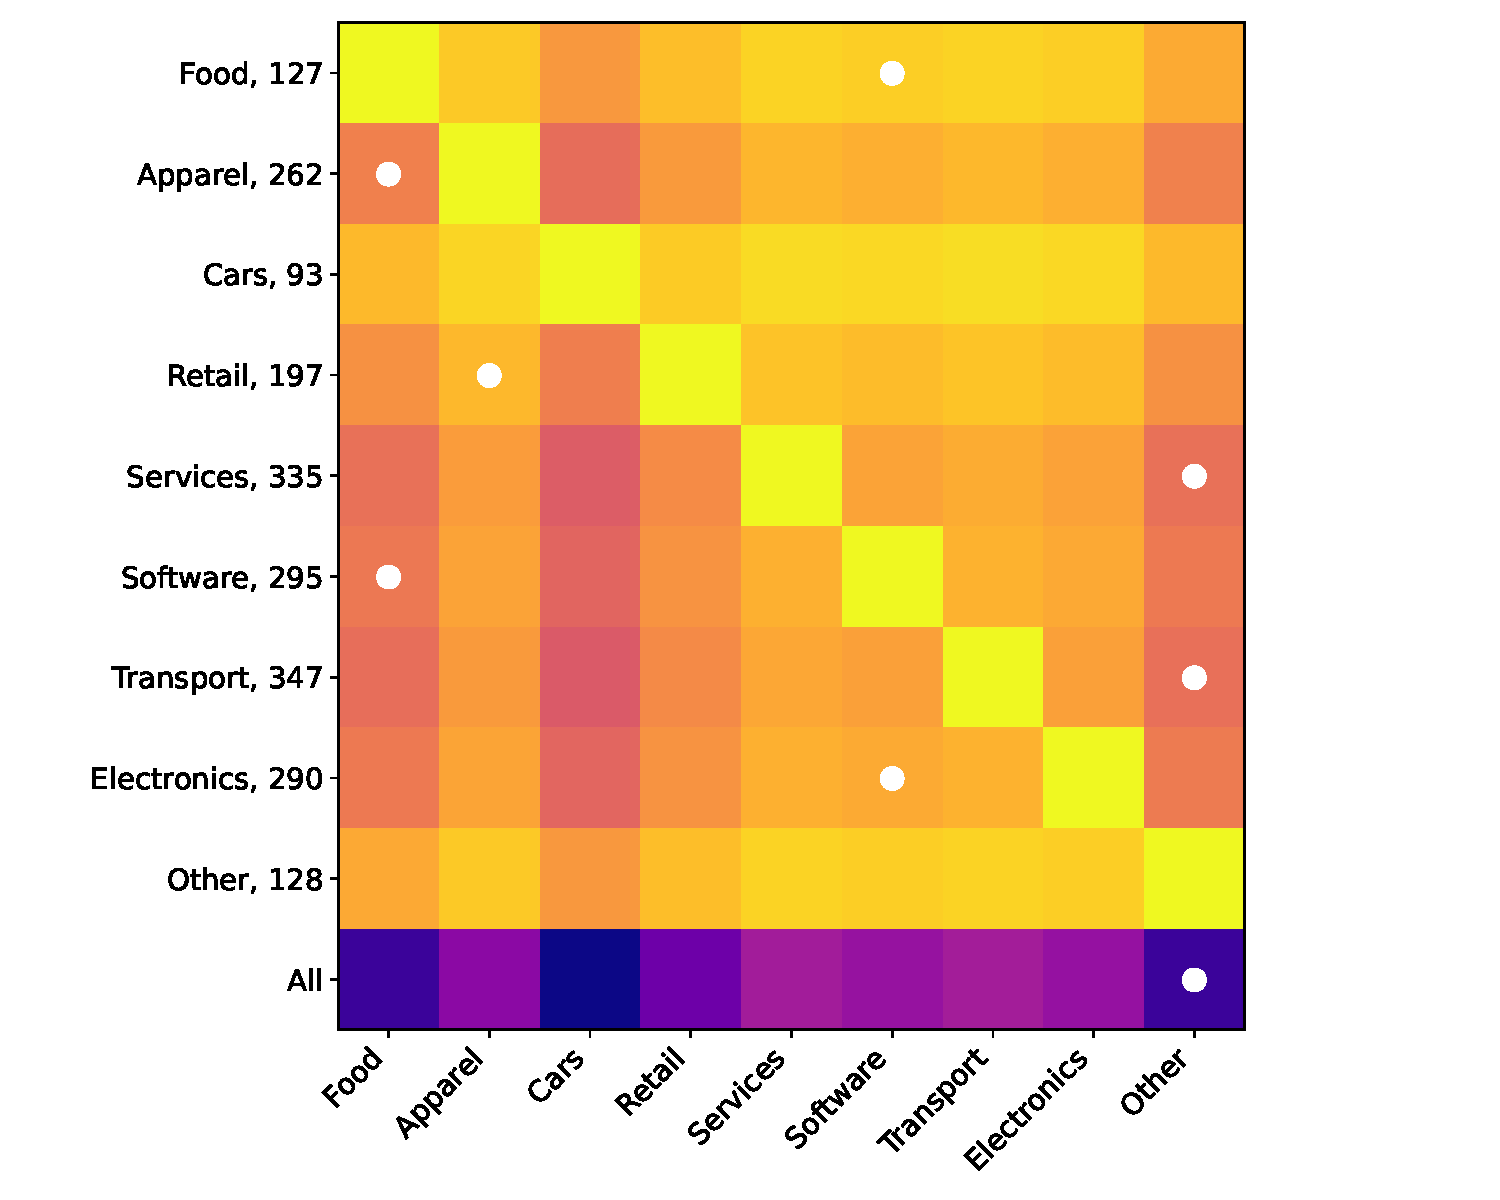
\includegraphics[width=9cm]{figures/cross_domain_data_heat.pdf}
    \vspace*{-3mm}
    \caption{Shows the heatmap of the log of the ratio of the train to test data for every combination executed during the experiments. The best-performing combination using AUC scores is highlighted with $\bullet$. Denoted next to the y-axis labels is the number of rows used for the train dataset for that domain.}
    \label{fig: cross_domain_heat}
\end{figure}